\section{逼真渲染和光线追踪算法}\label{sec:逼真渲染和光线追踪算法}

逼真渲染的目标是创建3D场景的图像且与同一场景的照片难以区分。
在我们介绍渲染流程之前要重点理解的是,
此处的{\itshape 难以区分}一词不是精确说法,
因为它涉及人类观察者,
不同观察者对同一图像的感知可能是不同的。
尽管本书会涉及少量感知问题,
但明确给出观察者的精确特性是非常困难且远未解决的问题。
绝大多数时候,我们都对针对光及其与物质相互作用的物理仿真感到满意,
并以我们对显示技术的理解尽可能向观察者展示最好的图像。

几乎所有逼真渲染系统都基于光线追踪算法。
光线追踪算法其实很简单;
它跟随光线\sidenote{译者注:原文a ray of light。
      此外会按个人理解把ray译作“光线”或“射线”,把light译作“光”或“光线”甚至“光源”。}路径
穿过场景与环境中的物体相互作用并反射。
虽然编写光线追踪器的方法有很多,
但所有这些系统都必须模拟至少一项以下对象和现象:
\begin{itemize}
      \item \keyindex{相机}{cameras}{camera相机}: 相机模型决定了从哪里、怎样观察场景,
            包括场景的图像是怎样记录到传感器上的。
            许多渲染系统从相机处开始生成视线并追踪到场景中。
      \item \keyindex{光线-物体交点}{ray–object intersections}{}: 此外,我们需要确定
            交点处物体的特定属性,例如曲面法线或材质。
            多数光线追踪器都有测试光线与多个物体相交的功能,
            典型的例如沿光线返回最近交点。
      \item \keyindex{光源}{light sources}{}: 没有光,渲染场景就没有意义。
            光线追踪器必须对整个场景的光分布建模,
            不仅包括灯光自身的位置,还包括它们向整个场景发散能量的方式。
      \item \keyindex{可见性}{visibility}{}:为了知道给定光是否在表面上一点积累能量,
            必须确认从该点到光源是否存在一条不中断的路径。
            幸运的是,在光线追踪器中这个问题很容易回答,
            因为我们可以构造从表面到光源\sidenote{译者注:原文为light,我按个人理解译作“光源”。}的射线,
            寻找最近的光线-物体交点,
            并比较交点距离和光源距离。
      \item \keyindex{表面散射}{surface scattering}{}:每个物体都必须提供外观描述,
            包括光如何与物体表面相互作用等信息,
            以及再辐射\sidenote{译者注:原文reradiated。}(或散射\sidenote{译者注:原文scattered。})光的性质。
            表面散射模型是典型的参数化模型,
            因此可以模拟各种外观。
      \item \keyindex{间接光传输}{indirect light transport}{light transport光传输}\sidenote{译者注:这里把transport译作“传输”是为了
                  与下一段propagation译作“传播”区分开,但个人理解似乎就是“传播”的意思。}:因为
            光在一个物体上反射或折射后可能遇到另一个物体,
            所以通常有必要追踪从表面发出的额外光线来捕捉这种效应。
      \item \keyindex{光线传播}{ray propagation}{}:我们需要知道光在空间中沿光线传播时发生了什么。
            如果渲染真空中的场景,则光能量沿光线保持恒定。
            真正的真空虽然在地球上是罕见的,
            但对许多环境而言是合理的近似。
            更多复杂模型可用于追踪穿过雾、烟、大气等的光线。
\end{itemize}

本节将简要讨论以上每个仿真任务。
后续章节会展示pbrt底层仿真组件的高级接口,
了解贯穿主渲染循环的单个光线处理过程。
我们还会介绍基于Turner Whitted的
原始光线追踪算法的表面散射模型实现。

\subsection{相机}\label{sub:相机}

几乎每个人都用过\keyindex{相机}{camera}{},熟悉它的基本功能:
你想用一张图像记下世界(通常是按按钮或点击屏幕),
然后图像就被记录到\keyindex{胶片}{film}{}或电子传感器上。
\keyindex{针孔相机}{pinhole camera}{camera相机}是最简单的拍照设备之一。
它由一端打有小孔的遮光盒组成(\reffig{1.1})。
当针孔未被遮挡时,光射进针孔落到固定在盒子另一端的相纸上。
虽然它很简单,但这种相机至今仍在使用,常用于艺术目的。
要在胶片上获得足够的光以形成图像需要非常长的曝光时间。
\begin{figure}
      \centering%LaTeX with PSTricks extensions
%%Creator: Inkscape 1.0.1 (3bc2e813f5, 2020-09-07)
%%Please note this file requires PSTricks extensions
\psset{xunit=.5pt,yunit=.5pt,runit=.5pt}
\begin{pspicture}(719.89001465,221.22999573)
{
\newrgbcolor{curcolor}{0 0 0}
\pscustom[linewidth=1,linecolor=curcolor]
{
\newpath
\moveto(180.38,220.31999573)
\lineto(54.38,140.19999573)
\lineto(54.38,1.18999573)
\lineto(180.38,81.30999573)
\closepath
}
}
{
\newrgbcolor{curcolor}{0 0 0}
\pscustom[linewidth=1,linecolor=curcolor]
{
\newpath
\moveto(393.38,220.31999573)
\lineto(267.38,140.19999573)
\lineto(267.38,1.18999573)
\lineto(393.38,81.30999573)
\closepath
}
}
{
\newrgbcolor{curcolor}{0 0 0}
\pscustom[linewidth=1,linecolor=curcolor]
{
\newpath
\moveto(180.02000427,220.5699957)
\lineto(393.23999023,220.5699957)
}
}
{
\newrgbcolor{curcolor}{0.72156864 0.70980394 0.70980394}
\pscustom[linestyle=none,fillstyle=solid,fillcolor=curcolor]
{
\newpath
\moveto(153.14,161.25999573)
\lineto(96.9,125.49999573)
\lineto(96.9,63.44999573)
\lineto(153.14,99.20999573)
\closepath
}
}
{
\newrgbcolor{curcolor}{0 0 0}
\pscustom[linewidth=1,linecolor=curcolor]
{
\newpath
\moveto(153.14,161.25999573)
\lineto(96.9,125.49999573)
\lineto(96.9,63.44999573)
\lineto(153.14,99.20999573)
\closepath
}
}
{
\newrgbcolor{curcolor}{0 0 0}
\pscustom[linewidth=1,linecolor=curcolor]
{
\newpath
\moveto(53.95000076,140.56999207)
\lineto(266.80999756,140.56999207)
}
}
{
\newrgbcolor{curcolor}{0 0 0}
\pscustom[linewidth=1,linecolor=curcolor]
{
\newpath
\moveto(180.02000427,82)
\lineto(393.58999634,82)
}
}
{
\newrgbcolor{curcolor}{0 0 0}
\pscustom[linewidth=1,linecolor=curcolor]
{
\newpath
\moveto(54.31000137,0.5)
\lineto(267.16000366,0.5)
}
}
{
\newrgbcolor{curcolor}{0 0 0}
\pscustom[linewidth=1,linecolor=curcolor]
{
\newpath
\moveto(339.7301427,119.158401)
\curveto(341.5742157,118.06695026)(341.46601021,114.47358161)(339.48845898,111.1323875)
\curveto(337.51090776,107.79119338)(334.41286921,105.96741604)(332.56879621,107.05886679)
\curveto(330.72472322,108.15031754)(330.8329287,111.74368618)(332.81047993,115.0848803)
\curveto(334.78803116,118.42607441)(337.88606971,120.24985175)(339.7301427,119.158401)
\closepath
}
}
{
\newrgbcolor{curcolor}{0 0 0}
\pscustom[linewidth=1,linecolor=curcolor]
{
\newpath
\moveto(576.36,162.31999573)
\lineto(520.12,126.55999573)
\lineto(520.12,64.50999573)
\lineto(576.36,100.26999573)
\closepath
}
}
{
\newrgbcolor{curcolor}{0 0 0}
\pscustom[linewidth=1,linecolor=curcolor]
{
\newpath
\moveto(153.71000671,161.95999527)
\lineto(631.82000732,33.97999573)
}
}
{
\newrgbcolor{curcolor}{0 0 0}
\pscustom[linewidth=1,linecolor=curcolor]
{
\newpath
\moveto(97.04000092,125.74999237)
\lineto(617.29998779,98.77999878)
}
}
{
\newrgbcolor{curcolor}{0 0 0}
\pscustom[linewidth=1,linecolor=curcolor]
{
\newpath
\moveto(96.43000031,63.16999817)
\lineto(673.23999023,182.71999741)
}
}
{
\newrgbcolor{curcolor}{0 0 0}
\pscustom[linewidth=1,linecolor=curcolor]
{
\newpath
\moveto(152.83999634,99.34999847)
\lineto(622.55999756,133.60999298)
}
}
{
\newrgbcolor{curcolor}{0 0 0}
\pscustom[linewidth=0.5,linecolor=curcolor]
{
\newpath
\moveto(379.01000977,47.37998962)
\lineto(338.20001221,103.22999573)
}
}
{
\newrgbcolor{curcolor}{0 0 0}
\pscustom[linewidth=0.5,linecolor=curcolor]
{
\newpath
\moveto(47.15000153,86.3999939)
\lineto(91.18000031,90.69999695)
}
}
{
\newrgbcolor{curcolor}{0 0 0}
\pscustom[linestyle=none,fillstyle=solid,fillcolor=curcolor]
{
\newpath
\moveto(369.586782,39.9484801)
\lineto(369.586782,41.0844801)
\lineto(366.242782,41.0844801)
\curveto(366.498782,41.5644801)(366.722782,42.0764801)(366.898782,42.5724801)
\lineto(365.842782,42.8924801)
\curveto(365.314782,41.4204801)(364.386782,39.9804801)(363.378782,39.0524801)
\curveto(363.570782,38.7964801)(363.890782,38.1884801)(363.986782,37.9484801)
\curveto(364.546782,38.5084801)(365.090782,39.1804801)(365.602782,39.9484801)
\closepath
\moveto(367.378782,30.4284801)
\lineto(367.378782,33.9644801)
\lineto(369.506782,33.9644801)
\lineto(369.506782,35.0524801)
\lineto(367.378782,35.0524801)
\lineto(367.378782,37.2124801)
\lineto(369.186782,37.2124801)
\lineto(369.186782,38.2844801)
\lineto(364.594782,38.2844801)
\lineto(364.594782,37.2124801)
\lineto(366.242782,37.2124801)
\lineto(366.242782,35.0524801)
\lineto(363.842782,35.0524801)
\lineto(363.842782,33.9644801)
\lineto(366.242782,33.9644801)
\lineto(366.242782,30.6524801)
\curveto(366.242782,29.9964801)(365.794782,29.6284801)(365.506782,29.4524801)
\curveto(365.714782,29.1964801)(365.970782,28.7004801)(366.066782,28.4124801)
\curveto(366.354782,28.6844801)(366.802782,28.9244801)(369.922782,30.5564801)
\curveto(369.842782,30.7964801)(369.746782,31.2604801)(369.714782,31.5804801)
\closepath
\moveto(378.034782,37.5964801)
\lineto(374.594782,37.5964801)
\lineto(374.594782,42.7964801)
\lineto(373.394782,42.7964801)
\lineto(373.394782,37.5964801)
\lineto(369.666782,37.5964801)
\lineto(369.666782,36.4284801)
\lineto(373.394782,36.4284801)
\lineto(373.394782,28.3324801)
\lineto(374.594782,28.3324801)
\lineto(374.594782,36.4284801)
\lineto(378.034782,36.4284801)
\closepath
}
}
{
\newrgbcolor{curcolor}{0 0 0}
\pscustom[linestyle=none,fillstyle=solid,fillcolor=curcolor]
{
\newpath
\moveto(386.62675148,42.0444801)
\lineto(386.38675148,41.9644801)
\lineto(379.77875148,41.9644801)
\lineto(379.77875148,40.8604801)
\lineto(385.47475148,40.8604801)
\curveto(384.77075148,40.0284801)(383.82675148,39.1324801)(382.97875148,38.5564801)
\lineto(382.97875148,35.4844801)
\curveto(381.61875148,35.1324801)(380.37075148,34.8124801)(379.42675148,34.5724801)
\lineto(379.68275148,33.3884801)
\lineto(382.97875148,34.3004801)
\lineto(382.97875148,29.8204801)
\curveto(382.97875148,29.5804801)(382.89875148,29.5164801)(382.64275148,29.5004801)
\curveto(382.41875148,29.5004801)(381.60275148,29.5004801)(380.70675148,29.5324801)
\curveto(380.89875148,29.1804801)(381.04275148,28.6684801)(381.09075148,28.3324801)
\curveto(382.25875148,28.3164801)(383.04275148,28.3484801)(383.52275148,28.5404801)
\curveto(383.98675148,28.7484801)(384.13075148,29.0844801)(384.13075148,29.8044801)
\lineto(384.13075148,34.6044801)
\lineto(387.37875148,35.5004801)
\lineto(387.21875148,36.6204801)
\curveto(386.19475148,36.3324801)(385.15475148,36.0444801)(384.13075148,35.7884801)
\lineto(384.13075148,38.0764801)
\curveto(385.29875148,38.9724801)(386.59475148,40.2684801)(387.42675148,41.4524801)
\closepath
\moveto(390.37075148,29.5484801)
\curveto(389.76275148,29.5484801)(389.63475148,29.6924801)(389.63475148,30.5084801)
\lineto(389.63475148,42.5564801)
\lineto(388.46675148,42.5564801)
\lineto(388.46675148,30.5404801)
\curveto(388.46675148,28.9244801)(388.83475148,28.4764801)(390.22675148,28.4764801)
\lineto(392.46675148,28.4764801)
\curveto(393.84275148,28.4764801)(394.14675148,29.3724801)(394.27475148,32.0124801)
\curveto(393.95475148,32.0924801)(393.49075148,32.3004801)(393.20275148,32.5404801)
\curveto(393.12275148,30.1404801)(393.02675148,29.5484801)(392.38675148,29.5484801)
\closepath
}
}
{
\newrgbcolor{curcolor}{0 0 0}
\pscustom[linestyle=none,fillstyle=solid,fillcolor=curcolor]
{
\newpath
\moveto(24.961985,91.8927451)
\lineto(20.801985,91.8927451)
\lineto(21.873985,92.3407451)
\curveto(21.665985,92.9167451)(21.153985,93.7167451)(20.641985,94.3087451)
\lineto(19.585985,93.8927451)
\curveto(20.081985,93.2847451)(20.545985,92.4527451)(20.769985,91.8927451)
\lineto(16.721985,91.8927451)
\lineto(16.721985,90.7887451)
\lineto(24.961985,90.7887451)
\closepath
\moveto(21.761985,89.8447451)
\curveto(22.769985,88.8047451)(23.953985,87.3487451)(24.449985,86.3887451)
\lineto(25.345985,87.1087451)
\curveto(24.817985,88.0527451)(23.617985,89.4447451)(22.593985,90.4527451)
\closepath
\moveto(18.641985,90.3727451)
\curveto(18.065985,89.2527451)(17.057985,87.9087451)(16.017985,87.0607451)
\curveto(16.273985,86.8687451)(16.641985,86.5487451)(16.833985,86.3407451)
\curveto(17.889985,87.2847451)(18.977985,88.6287451)(19.681985,89.9087451)
\closepath
\moveto(12.801985,85.9247451)
\curveto(12.817985,86.5807451)(12.833985,87.2367451)(12.833985,87.8127451)
\lineto(12.833985,88.6767451)
\lineto(14.849985,88.6767451)
\lineto(14.849985,85.9247451)
\closepath
\moveto(14.849985,92.4047451)
\lineto(14.849985,89.7487451)
\lineto(12.833985,89.7487451)
\lineto(12.833985,92.4047451)
\closepath
\moveto(15.937985,93.4767451)
\lineto(11.777985,93.4767451)
\lineto(11.777985,87.7967451)
\curveto(11.777985,85.4607451)(11.697985,82.3247451)(10.641985,80.1007451)
\curveto(10.913985,79.9887451)(11.377985,79.7167451)(11.585985,79.5247451)
\curveto(12.289985,81.0447451)(12.593985,82.9967451)(12.737985,84.8367451)
\lineto(14.849985,84.8367451)
\lineto(14.849985,81.0767451)
\curveto(14.849985,80.8847451)(14.785985,80.8367451)(14.609985,80.8207451)
\curveto(14.465985,80.8207451)(13.921985,80.8047451)(13.361985,80.8367451)
\curveto(13.505985,80.5487451)(13.665985,80.0527451)(13.697985,79.7487451)
\curveto(14.545985,79.7487451)(15.089985,79.7807451)(15.441985,79.9727451)
\curveto(15.809985,80.1647451)(15.937985,80.4847451)(15.937985,81.0767451)
\closepath
\moveto(22.449985,87.5407451)
\curveto(22.081985,86.2127451)(21.489985,85.0127451)(20.689985,83.9727451)
\curveto(19.873985,85.0127451)(19.233985,86.2127451)(18.769985,87.5087451)
\lineto(17.745985,87.2207451)
\curveto(18.273985,85.6847451)(19.009985,84.2927451)(19.937985,83.1087451)
\curveto(18.865985,82.0207451)(17.521985,81.1567451)(15.921985,80.4687451)
\curveto(16.161985,80.2767451)(16.513985,79.8447451)(16.673985,79.5887451)
\curveto(18.257985,80.2767451)(19.585985,81.1567451)(20.673985,82.2447451)
\curveto(21.761985,81.1247451)(23.041985,80.2447451)(24.545985,79.6527451)
\curveto(24.721985,79.9887451)(25.073985,80.4527451)(25.345985,80.7087451)
\curveto(23.841985,81.2047451)(22.545985,82.0367451)(21.457985,83.1247451)
\curveto(22.417985,84.2927451)(23.121985,85.6527451)(23.585985,87.2527451)
\closepath
}
}
{
\newrgbcolor{curcolor}{0 0 0}
\pscustom[linestyle=none,fillstyle=solid,fillcolor=curcolor]
{
\newpath
\moveto(30.22595448,88.9167451)
\lineto(40.48195448,88.9167451)
\lineto(40.48195448,90.1167451)
\lineto(36.00195448,90.1167451)
\lineto(36.00195448,94.2127451)
\lineto(34.75395448,94.2127451)
\lineto(34.75395448,90.1167451)
\lineto(30.22595448,90.1167451)
\lineto(30.22595448,93.8127451)
\lineto(29.00995448,93.8127451)
\lineto(29.00995448,88.5167451)
\curveto(29.00995448,85.7327451)(28.78595448,82.7887451)(26.76995448,80.5327451)
\curveto(27.04195448,80.3247451)(27.48995448,79.8927451)(27.68195448,79.6047451)
\curveto(29.15395448,81.2207451)(29.77795448,83.1567451)(30.03395448,85.1567451)
\lineto(36.75395448,85.1567451)
\lineto(36.75395448,79.6367451)
\lineto(38.01795448,79.6367451)
\lineto(38.01795448,86.3727451)
\lineto(30.16195448,86.3727451)
\curveto(30.20995448,87.0927451)(30.22595448,87.8127451)(30.22595448,88.5327451)
\closepath
}
}
{
\newrgbcolor{curcolor}{0 0 0}
\pscustom[linestyle=none,fillstyle=solid,fillcolor=curcolor]
{
\newpath
\moveto(635.912685,116.5621301)
\lineto(640.824685,116.5621301)
\lineto(640.824685,109.1701301)
\lineto(642.008685,109.1701301)
\lineto(642.008685,117.6181301)
\lineto(634.760685,117.6181301)
\lineto(634.760685,109.1701301)
\lineto(635.912685,109.1701301)
\closepath
\moveto(632.488685,116.3541301)
\curveto(632.200685,116.9461301)(631.576685,117.7621301)(630.968685,118.3541301)
\lineto(630.056685,117.8261301)
\curveto(630.632685,117.2021301)(631.240685,116.3221301)(631.528685,115.7461301)
\closepath
\moveto(634.056685,109.4741301)
\curveto(633.752685,109.8261301)(632.648685,111.1061301)(632.056685,111.7621301)
\curveto(632.808685,112.8341301)(633.464685,114.0501301)(633.912685,115.2661301)
\lineto(633.272685,115.6981301)
\lineto(633.048685,115.6501301)
\lineto(628.616685,115.6501301)
\lineto(628.616685,114.5621301)
\lineto(632.472685,114.5621301)
\curveto(631.544685,112.5461301)(629.848685,110.5461301)(628.232685,109.4421301)
\curveto(628.408685,109.2181301)(628.664685,108.6261301)(628.760685,108.2901301)
\curveto(629.384685,108.7541301)(630.008685,109.3301301)(630.616685,109.9861301)
\lineto(630.616685,103.7941301)
\lineto(631.752685,103.7941301)
\lineto(631.752685,110.6421301)
\curveto(632.312685,109.9221301)(632.984685,109.0101301)(633.304685,108.5301301)
\closepath
\moveto(639.944685,104.9301301)
\curveto(639.480685,104.9301301)(639.352685,105.0421301)(639.352685,105.4901301)
\lineto(639.352685,109.4261301)
\lineto(638.552685,109.4261301)
\curveto(638.792685,110.4021301)(638.872685,111.3301301)(638.872685,112.2101301)
\lineto(638.872685,115.3461301)
\lineto(637.720685,115.3461301)
\lineto(637.720685,112.2421301)
\curveto(637.720685,109.7621301)(637.240685,106.7381301)(633.224685,104.6581301)
\curveto(633.464685,104.4661301)(633.848685,104.0181301)(633.976685,103.7621301)
\curveto(636.360685,105.0261301)(637.608685,106.7061301)(638.248685,108.4181301)
\lineto(638.248685,105.3621301)
\curveto(638.248685,104.3221301)(638.680685,104.0181301)(639.768685,104.0181301)
\lineto(641.224685,104.0181301)
\curveto(642.584685,104.0181301)(642.776685,104.6581301)(642.920685,107.1701301)
\curveto(642.616685,107.2501301)(642.232685,107.4101301)(641.944685,107.6341301)
\curveto(641.864685,105.3461301)(641.784685,104.9301301)(641.240685,104.9301301)
\closepath
}
}
{
\newrgbcolor{curcolor}{0 0 0}
\pscustom[linestyle=none,fillstyle=solid,fillcolor=curcolor]
{
\newpath
\moveto(646.44065448,117.5061301)
\lineto(646.44065448,108.4341301)
\lineto(647.65665448,108.4341301)
\lineto(647.65665448,116.3221301)
\lineto(655.35265448,116.3221301)
\lineto(655.35265448,108.4341301)
\lineto(656.60065448,108.4341301)
\lineto(656.60065448,117.5061301)
\closepath
\moveto(650.79265448,114.8341301)
\curveto(650.64865448,109.2181301)(650.42465448,106.1781301)(644.36065448,104.8021301)
\curveto(644.58465448,104.5621301)(644.92065448,104.0821301)(645.03265448,103.7781301)
\curveto(651.43265448,105.3461301)(651.84865448,108.8021301)(652.02465448,114.8341301)
\closepath
\moveto(651.81665448,109.7941301)
\lineto(651.81665448,105.8261301)
\curveto(651.81665448,104.5141301)(652.29665448,104.1781301)(653.83265448,104.1781301)
\lineto(656.68065448,104.1781301)
\curveto(658.12065448,104.1781301)(658.48865448,104.7701301)(658.63265448,107.2501301)
\curveto(658.31265448,107.3301301)(657.81665448,107.5221301)(657.54465448,107.7301301)
\curveto(657.46465448,105.5861301)(657.35265448,105.2821301)(656.58465448,105.2821301)
\lineto(653.92865448,105.2821301)
\curveto(653.14465448,105.2821301)(652.98465448,105.3621301)(652.98465448,105.8421301)
\lineto(652.98465448,109.7941301)
\closepath
}
}
{
\newrgbcolor{curcolor}{0 0 0}
\pscustom[linestyle=none,fillstyle=solid,fillcolor=curcolor]
{
\newpath
\moveto(663.60862396,118.3381301)
\curveto(662.80862396,115.9221301)(661.51262396,113.5381301)(660.10462396,111.9861301)
\curveto(660.31262396,111.7141301)(660.66462396,111.0901301)(660.79262396,110.8181301)
\curveto(661.25662396,111.3621301)(661.72062396,111.9861301)(662.15262396,112.6581301)
\lineto(662.15262396,103.8101301)
\lineto(663.28862396,103.8101301)
\lineto(663.28862396,114.6261301)
\curveto(663.83262396,115.7141301)(664.32862396,116.8661301)(664.71262396,118.0021301)
\closepath
\moveto(674.74462396,114.0341301)
\lineto(674.74462396,115.1861301)
\lineto(669.97662396,115.1861301)
\lineto(669.97662396,118.3381301)
\lineto(668.82462396,118.3381301)
\lineto(668.82462396,115.1861301)
\lineto(664.34462396,115.1861301)
\lineto(664.34462396,114.0341301)
\lineto(668.10462396,114.0341301)
\curveto(667.12862396,111.3301301)(665.46462396,108.6421301)(663.72062396,107.2341301)
\curveto(663.99262396,107.0261301)(664.37662396,106.6101301)(664.58462396,106.3381301)
\curveto(666.26462396,107.8741301)(667.80062396,110.4981301)(668.82462396,113.2661301)
\lineto(668.82462396,107.8261301)
\lineto(666.21662396,107.8261301)
\lineto(666.21662396,106.7381301)
\lineto(668.82462396,106.7381301)
\lineto(668.82462396,103.8741301)
\lineto(669.97662396,103.8741301)
\lineto(669.97662396,106.7381301)
\lineto(672.55262396,106.7381301)
\lineto(672.55262396,107.8261301)
\lineto(669.97662396,107.8261301)
\lineto(669.97662396,113.3781301)
\curveto(670.95262396,110.5941301)(672.48862396,107.9061301)(674.16862396,106.3701301)
\curveto(674.37662396,106.6901301)(674.77662396,107.1061301)(675.06462396,107.3141301)
\curveto(673.33662396,108.7061301)(671.68862396,111.3621301)(670.74462396,114.0341301)
\closepath
}
}
\end{pspicture}

      \caption{针孔相机}\label{fig:1.1}
\end{figure}

虽然大多数相机都比针孔相机复杂得多,
但针孔相机是仿真的便捷起点。
相机最重要的功能是定义会被记录到胶片上的场景部分。
在\reffig{1.1}中,我们可以看见从针孔到胶片边的连线
是如何构造出延伸到场景中的双锥体的。
不在该锥体内的物体不会在胶片上成像。
因为实际的相机成像形状比锥体更复杂,
所以我们把这个可能在胶片上成像的空间区域称为\keyindex{视见体}{viewing volume}{}。

针孔相机也可以看作是把胶片平面放置在针孔的\emph{前方}但距离不变(\reffig{1.2})。
注意从针孔到胶片的连线正好定义了和之前一样的视见体。
当然,这不是真实相机的实际构建方法,
但对于仿真目的而言它是个方便的抽象。
当胶片(或成像)平面在针孔前时,
针孔也常常改称作\keyindex{眼睛}{eye}{}。
\begin{figure}
      \centering%LaTeX with PSTricks extensions
%%Creator: Inkscape 1.0.1 (3bc2e813f5, 2020-09-07)
%%Please note this file requires PSTricks extensions
\psset{xunit=.5pt,yunit=.5pt,runit=.5pt}
\begin{pspicture}(330.91000366,165.99000549)
{
\newrgbcolor{curcolor}{0 0 0}
\pscustom[linewidth=1,linecolor=curcolor]
{
\newpath
\moveto(67.98000336,94.66000366)
\lineto(330.86999512,75.11000824)
}
}
{
\newrgbcolor{curcolor}{0 0 0}
\pscustom[linewidth=1,linecolor=curcolor]
{
\newpath
\moveto(68.19999695,94.96000671)
\lineto(302.67001343,0.46000671)
}
}
{
\newrgbcolor{curcolor}{0.72156864 0.70980394 0.70980394}
\pscustom[linestyle=none,fillstyle=solid,fillcolor=curcolor]
{
\newpath
\moveto(248.69,143.30000549)
\lineto(192.44,107.54000549)
\lineto(192.44,45.49000549)
\lineto(248.69,81.25000549)
\closepath
}
}
{
\newrgbcolor{curcolor}{0 0 0}
\pscustom[linewidth=1,linecolor=curcolor]
{
\newpath
\moveto(248.69,143.30000549)
\lineto(192.44,107.54000549)
\lineto(192.44,45.49000549)
\lineto(248.69,81.25000549)
\closepath
}
}
{
\newrgbcolor{curcolor}{0 0 0}
\pscustom[linewidth=1,linecolor=curcolor]
{
\newpath
\moveto(68.48000336,94.91000366)
\lineto(330.27999878,121.91000366)
}
}
{
\newrgbcolor{curcolor}{0 0 0}
\pscustom[linewidth=1,linecolor=curcolor]
{
\newpath
\moveto(68.19999695,95.15000916)
\lineto(327.17999268,165.5100055)
}
}
{
\newrgbcolor{curcolor}{0.73333335 0.74117649 0.74901962}
\pscustom[linestyle=none,fillstyle=solid,fillcolor=curcolor]
{
\newpath
\moveto(42.85,111.07000549)
\curveto(49.67,99.89000549)(48.24,89.56000549)(38.92,82.39000549)
\curveto(26.86,92.99000549)(14.6,97.78000549)(5.46,100.99000549)
\curveto(5.85,100.99000549)(6.24,101.06000549)(6.65,101.10000549)
\curveto(17.81,102.23000549)(29.33,103.34000549)(42.85,111.07000549)
\closepath
}
}
{
\newrgbcolor{curcolor}{0 0 0}
\pscustom[linestyle=none,fillstyle=solid,fillcolor=curcolor]
{
\newpath
\moveto(38.92,82.39000549)
\curveto(48.24,89.56000549)(49.67,99.89000549)(42.85,111.07000549)
\curveto(29.33,103.34000549)(17.85,102.23000549)(6.65,101.14000549)
\curveto(6.24,101.14000549)(5.85,101.08000549)(5.46,101.03000549)
\curveto(14.6,97.78000549)(26.86,92.99000549)(38.92,82.39000549)
\closepath
\moveto(44.77,112.21000549)
\curveto(52.03,100.21000549)(50.49,88.68000549)(40.61,80.86000549)
\curveto(42.08,79.51000549)(43.55,78.09000549)(45,76.55000549)
\lineto(43.37,74.99000549)
\curveto(28.71,90.54000549)(12.75,96.11000549)(2.19,99.79000549)
\lineto(0,100.58000549)
\curveto(-1.76754134,97.580174)(-6.32632363,99.74115465)(-5.15315982,102.99994303)
\curveto(-3.979996,106.2587314)(0.91011569,105.01811022)(0.36,101.58000549)
\curveto(0.02896037,97.84195685)(-5.409727,97.83838194)(-5.77137565,101.5534999)
\curveto(-6.1330243,105.26861786)(-0.79575471,106.31402991)(0.25,102.71000549)
\curveto(2.33,102.93000549)(4.37,103.15000549)(6.42,103.34000549)
\curveto(19.66,104.62000549)(32.17,105.80000549)(48.16,117.06000549)
\lineto(49.44,115.24000549)
\curveto(47.86,114.15000549)(46.3,113.15000549)(44.77,112.21000549)
\closepath
}
}
{
\newrgbcolor{curcolor}{1 1 1}
\pscustom[linestyle=none,fillstyle=solid,fillcolor=curcolor]
{
\newpath
\moveto(45.7,95.68000549)
\curveto(44.94,90.87000549)(41.84,87.36000549)(38.79,87.85000549)
\curveto(35.74,88.34000549)(33.88,92.64000549)(34.65,97.44000549)
\curveto(35.42,102.24000549)(38.51,105.77000549)(41.57,105.28000549)
\curveto(44.63,104.79000549)(46.48,100.50000549)(45.7,95.68000549)
\closepath
}
}
{
\newrgbcolor{curcolor}{0.12941177 0.12941177 0.12941177}
\pscustom[linestyle=none,fillstyle=solid,fillcolor=curcolor]
{
\newpath
\moveto(44.66,94.85000549)
\curveto(45.10896351,97.9766758)(41.54030622,100.07343854)(39.02747808,98.16011762)
\curveto(36.51464993,96.2467967)(37.5865553,92.24895382)(40.72,91.85000549)
\curveto(42.90474114,91.0470233)(45.29252279,92.37351826)(45.76503229,94.65268173)
\curveto(46.23754179,96.93184519)(44.57390184,99.09826902)(42.25,99.23000549)
\curveto(39.21982147,100.11379445)(36.63602428,96.89026441)(38.15746695,94.12515283)
\curveto(39.67890962,91.36004126)(43.7847623,91.81734597)(44.66,94.85000549)
\closepath
}
}
{
\newrgbcolor{curcolor}{0 0 0}
\pscustom[linestyle=none,fillstyle=solid,fillcolor=curcolor]
{
\newpath
\moveto(249.84836175,59.90126994)
\lineto(245.68836175,59.90126994)
\lineto(246.76036175,60.34926994)
\curveto(246.55236175,60.92526994)(246.04036175,61.72526994)(245.52836175,62.31726994)
\lineto(244.47236175,61.90126994)
\curveto(244.96836175,61.29326994)(245.43236175,60.46126994)(245.65636175,59.90126994)
\lineto(241.60836175,59.90126994)
\lineto(241.60836175,58.79726994)
\lineto(249.84836175,58.79726994)
\closepath
\moveto(246.64836175,57.85326994)
\curveto(247.65636175,56.81326994)(248.84036175,55.35726994)(249.33636175,54.39726994)
\lineto(250.23236175,55.11726994)
\curveto(249.70436175,56.06126994)(248.50436175,57.45326994)(247.48036175,58.46126994)
\closepath
\moveto(243.52836175,58.38126994)
\curveto(242.95236175,57.26126994)(241.94436175,55.91726994)(240.90436175,55.06926994)
\curveto(241.16036175,54.87726994)(241.52836175,54.55726994)(241.72036175,54.34926994)
\curveto(242.77636175,55.29326994)(243.86436175,56.63726994)(244.56836175,57.91726994)
\closepath
\moveto(237.68836175,53.93326994)
\curveto(237.70436175,54.58926994)(237.72036175,55.24526994)(237.72036175,55.82126994)
\lineto(237.72036175,56.68526994)
\lineto(239.73636175,56.68526994)
\lineto(239.73636175,53.93326994)
\closepath
\moveto(239.73636175,60.41326994)
\lineto(239.73636175,57.75726994)
\lineto(237.72036175,57.75726994)
\lineto(237.72036175,60.41326994)
\closepath
\moveto(240.82436175,61.48526994)
\lineto(236.66436175,61.48526994)
\lineto(236.66436175,55.80526994)
\curveto(236.66436175,53.46926994)(236.58436175,50.33326994)(235.52836175,48.10926994)
\curveto(235.80036175,47.99726994)(236.26436175,47.72526994)(236.47236175,47.53326994)
\curveto(237.17636175,49.05326994)(237.48036175,51.00526994)(237.62436175,52.84526994)
\lineto(239.73636175,52.84526994)
\lineto(239.73636175,49.08526994)
\curveto(239.73636175,48.89326994)(239.67236175,48.84526994)(239.49636175,48.82926994)
\curveto(239.35236175,48.82926994)(238.80836175,48.81326994)(238.24836175,48.84526994)
\curveto(238.39236175,48.55726994)(238.55236175,48.06126994)(238.58436175,47.75726994)
\curveto(239.43236175,47.75726994)(239.97636175,47.78926994)(240.32836175,47.98126994)
\curveto(240.69636175,48.17326994)(240.82436175,48.49326994)(240.82436175,49.08526994)
\closepath
\moveto(247.33636175,55.54926994)
\curveto(246.96836175,54.22126994)(246.37636175,53.02126994)(245.57636175,51.98126994)
\curveto(244.76036175,53.02126994)(244.12036175,54.22126994)(243.65636175,55.51726994)
\lineto(242.63236175,55.22926994)
\curveto(243.16036175,53.69326994)(243.89636175,52.30126994)(244.82436175,51.11726994)
\curveto(243.75236175,50.02926994)(242.40836175,49.16526994)(240.80836175,48.47726994)
\curveto(241.04836175,48.28526994)(241.40036175,47.85326994)(241.56036175,47.59726994)
\curveto(243.14436175,48.28526994)(244.47236175,49.16526994)(245.56036175,50.25326994)
\curveto(246.64836175,49.13326994)(247.92836175,48.25326994)(249.43236175,47.66126994)
\curveto(249.60836175,47.99726994)(249.96036175,48.46126994)(250.23236175,48.71726994)
\curveto(248.72836175,49.21326994)(247.43236175,50.04526994)(246.34436175,51.13326994)
\curveto(247.30436175,52.30126994)(248.00836175,53.66126994)(248.47236175,55.26126994)
\closepath
}
}
{
\newrgbcolor{curcolor}{0 0 0}
\pscustom[linestyle=none,fillstyle=solid,fillcolor=curcolor]
{
\newpath
\moveto(255.11233123,56.92526994)
\lineto(265.36833123,56.92526994)
\lineto(265.36833123,58.12526994)
\lineto(260.88833123,58.12526994)
\lineto(260.88833123,62.22126994)
\lineto(259.64033123,62.22126994)
\lineto(259.64033123,58.12526994)
\lineto(255.11233123,58.12526994)
\lineto(255.11233123,61.82126994)
\lineto(253.89633123,61.82126994)
\lineto(253.89633123,56.52526994)
\curveto(253.89633123,53.74126994)(253.67233123,50.79726994)(251.65633123,48.54126994)
\curveto(251.92833123,48.33326994)(252.37633123,47.90126994)(252.56833123,47.61326994)
\curveto(254.04033123,49.22926994)(254.66433123,51.16526994)(254.92033123,53.16526994)
\lineto(261.64033123,53.16526994)
\lineto(261.64033123,47.64526994)
\lineto(262.90433123,47.64526994)
\lineto(262.90433123,54.38126994)
\lineto(255.04833123,54.38126994)
\curveto(255.09633123,55.10126994)(255.11233123,55.82126994)(255.11233123,56.54126994)
\closepath
}
}
\end{pspicture}

      \caption{当仿真针孔相机时,胶片放在针孔前的平面,针孔改称为\emph{眼睛}。}\label{fig:1.2}
\end{figure}

现在我们说到渲染的关键问题:
相机在图像中的每一点记录下的颜色值是什么?
回想最初的针孔相机,
显然光线只有沿着连接针孔与胶片上一点的向量
传播才能作用于胶片上的相应位置。
在把胶片放在眼睛前的仿真相机中,
我们关注沿着图像点传播到眼睛的
光量\sidenote{译者注:原文the amount of light,
      即“光的数量”。这里译为“光量”,可以笼统理解为光的强弱。}。

因此,相机仿真器的重要任务是取图像上一点
并生成\keyindex{射线}{ray}{},
沿这些射线的\keyindex{入射光}{incident light}{light光}可作用于该图像位置。
因为射线由一个\keyindex{端点}{origin point}{point点}和
一个\keyindex{方向向量}{direction vector}{vector向量}组成,
所以该任务对\reffig{1.2}的针孔相机而言很简单:
它把针孔作为端点,
把从针孔到像平面\sidenote{译者注:原文near plane,按
      个人理解改译为“像平面”。}的向量
作为射线的方向。
对于含有多个透镜的复杂相机模型,
则图像上给定点相应的射线需要更多计算
(\refsec{逼真相机}介绍了这类模型的实现)。


\subsection{光线-物体交点}\label{sub:光线-物体交点}

相机每次生成射线时,
渲染器第一个任务就是确定
如果有的话,哪个物体和该射线最先\keyindex{相交}{intersect}{},
交点在哪里。
该\keyindex{交点}{intersection point}{point点}是沿射线可见的,
我们想要模拟光在该点与物体的相互作用。
为了找到交点,我们必须把场景中的所有物体拿来和该射线测试,
并选出与该射线首先相交的那个。
给定一射线$\mathrm{r}$,首先将其写成\keyindex{参数形式}{parametric form}{}:
\begin{align*}
      \mathrm{r}(t)=\mathrm{o}+t\mathbf{d}\, ,
\end{align*}
其中$\mathrm{o}$是射线端点,$\mathbf{d}$是其方向向量,$t$是定义在$(0,\infty)$的\keyindex{参数}{parameter}{}。
我们可以通过指定参数$t$的值并代入上式求得射线上的一点。

通常很容易寻找射线$\mathrm{r}$和由隐函数$F(x,y,z)=0$定义的\keyindex{曲面}{surface}{}的交点。
首先把射线方程代入\keyindex{隐式方程}{implicit equation}{equation方程},
得到只含有参数$t$的新方程。
然后从中解出$t$并把最小正根代入射线方程得到所需的点。
例如,以\keyindex{原点}{origin}{point点}为球心,$r$为\keyindex{半径}{radius}{}的\keyindex{球}{sphere}{}的隐式方程是
\begin{align*}
      x^2+y^2+z^2-r^2=0\, .
\end{align*}
代入射线方程,得到
\begin{align*}
      (\mathrm{o}_x+t\mathbf{d}_x)^2+(\mathrm{o}_y+t\mathbf{d}_y)^2+(\mathrm{o}_z+t\mathbf{d}_z)^2-r^2=0\, .
\end{align*}
上式除了$t$外的所有值都是已知的,因此是易解的关于$t$的二次方程。
如果没有正根,则射线与球面错开了;
如果有,则最小正根给出了交点。

对于光线追踪器的其余部分。只有交点信息是不够的;
它还需要知道该点表明的特定属性。
首先,必须确定该点的材质表示
并传给光线追踪算法之后的步骤。
其次,还需要交点处额外的几何信息来对该点\keyindex{着色}{shade}{}。
例如,曲面\keyindex{法线}{normal}{}$\mathbf{n}$是必需的。
虽然许多光线追踪器只对$\mathbf{n}$操作,
但像pbrt这类更复杂的渲染系统还需要更多信息,
比如位置的各个\keyindex{偏导数}{partial derivative}{derivative导数}以及
关于曲面局部参数化的曲面法线。

当然,绝大多数场景含有多个物体。
暴力法指依次用每个物体对射线测试,
从所有交点中选出$t$的最小正值来求得最近交点。
该方法虽然正确但对哪怕适度复杂的场景也很慢。
更好的方法是在射线交点处理中
并入一个\keyindex{加速结构}{acceleration structure}{}快速否决整组物体。
快速剔除无关几何体的能力意味着光线追踪常能以$O(I\log{N})$的时间运行,
其中$I$是图像像素数目,
$N$是场景中物体的数量
(然而构建加速结构本身至少需要$O(N)$时间)。
\begin{remark}
      虽然光线追踪的对数复杂度是
      常被认为是其主要优点,但该复杂度只在平均意义下是典型正确的。
      在计算几何文献中发表的许多光线追踪算法都保证有对数运行时间,
      但它们只在特定种类场景下才能工作,并且预处理开销和存储要求很高。
      Szirmay-Kalos和Márton提供了相关参考文献\citep{10.1007/BF02684409}
      {\itshape (译者注:原文缺失该引文标注,本人推测为该文)}。
      但好在表现真实环境的场景通常不会遇到这种最坏的情形。
      实践中本书介绍的射线相交算法是次线性的,
      但在去掉大量预处理和存储开销时
      总是有可能构造出使光线追踪以$O(IN)$时间运行的最坏情形。
\end{remark}

pbrt为各种形状实现的几何接口将在第\refchap{形状}介绍,
加速接口和实现在第\refchap{图元和交点加速}说明。

\subsection{光分布}\label{sub:光分布}

光线-物体交点阶段给出了要着色的点和该点的局部几何信息。
回想我们的最终目标是找出从该点出发朝相机方向传播的光量。
为此需要知道有多少光\emph{到达}了该点。
这同时涉及到场景中光的\emph{几何}和\emph{辐射}分布。
对于非常简单的光源(例如\keyindex{点光源}{point light}{light sources光源}),
光的\keyindex{几何分布}{geometric distribution}{distribution分布}只需
知道光源位置即可。
然而真实世界并不存在点光源,
所以基于物理的光照常基于\keyindex{面光源}{area light sources}{light sources光源}。
这意味着光源和表面发光的几何体关联。
但本节我们用点光源说明光分布的构成;
光度量和分布的严格讨论是第\refchap{颜色和辐射学}和第\refchap{光源}的主题。

我们常常想知道光在交点附近的微分面积上积累的功率(\reffig{1.3})。
假设点光源具有功率\sidenote{译者注:称为辐射通量或辐射功率。}
$\varPhi$并向所有方向均匀辐射光
\sidenote{译者注:原文使用正体字母$\Phi$,
      我把标量统一改为了斜体;
      此外原文正确使用了$\pi$的正体表示圆周率,
      但我因为字体环境冲突无法打出正体,
      所以全书被迫用的斜体。}。
这意味着围绕光源的单位球面在单位面积上的功率
为$\displaystyle\frac{\varPhi}{4\mathrm{\pi}}$
(这些度量将在\refsec{辐射学}解释和形式化)。
\begin{figure}
      \centering%LaTeX with PSTricks extensions
%%Creator: Inkscape 1.0.1 (3bc2e813f5, 2020-09-07)
%%Please note this file requires PSTricks extensions
\psset{xunit=.5pt,yunit=.5pt,runit=.5pt}
\begin{pspicture}(435.51000977,280.66000366)
{
\newrgbcolor{curcolor}{0 0 0}
\pscustom[linewidth=0.5,linecolor=curcolor]
{
\newpath
\moveto(435.09,186.74000366)
\lineto(98.11,188.58000366)
\lineto(0.41,2.09000366)
\lineto(337.39,0.25000366)
\closepath
}
}
{
\newrgbcolor{curcolor}{0 0 0}
\pscustom[linewidth=1,linecolor=curcolor]
{
\newpath
\moveto(217.75,94.80000305)
\lineto(217.75,264.30000305)
}
}
{
\newrgbcolor{curcolor}{0 0 0}
\pscustom[linestyle=none,fillstyle=solid,fillcolor=curcolor]
{
\newpath
\moveto(220.5,261.85000366)
\lineto(217.75,263.98000366)
\lineto(215,261.85000366)
\lineto(217.75,268.36000366)
\closepath
}
}
{
\newrgbcolor{curcolor}{0.65098041 0.65098041 0.65098041}
\pscustom[linestyle=none,fillstyle=solid,fillcolor=curcolor]
{
\newpath
\moveto(219.9,262.63000366)
\lineto(217.75,267.70000366)
\lineto(217.75,264.29000366)
\closepath
}
}
{
\newrgbcolor{curcolor}{0.40000001 0.40000001 0.40000001}
\pscustom[linestyle=none,fillstyle=solid,fillcolor=curcolor]
{
\newpath
\moveto(215.6,262.63000366)
\lineto(217.75,267.70000366)
\lineto(217.75,264.29000366)
\closepath
}
}
{
\newrgbcolor{curcolor}{0 0 0}
\pscustom[linestyle=none,fillstyle=solid,fillcolor=curcolor]
{
\newpath
\moveto(219.88000488,95.08999634)
\curveto(219.88000488,97.09467166)(217.45644314,98.09825347)(216.03909545,96.68090578)
\curveto(214.62174775,95.26355808)(215.62532956,92.83999634)(217.63000488,92.83999634)
\curveto(219.63468021,92.83999634)(220.63826201,95.26355808)(219.22091432,96.68090578)
\curveto(217.80356663,98.09825347)(215.38000488,97.09467166)(215.38000488,95.08999634)
\curveto(215.38000488,93.08532101)(217.80356663,92.08173921)(219.22091432,93.4990869)
\curveto(220.63826201,94.91643459)(219.63468021,97.33999634)(217.63000488,97.33999634)
\curveto(215.62532956,97.33999634)(214.62174775,94.91643459)(216.03909545,93.4990869)
\curveto(217.45644314,92.08173921)(219.88000488,93.08532101)(219.88000488,95.08999634)
\closepath
}
}
{
\newrgbcolor{curcolor}{0 0 0}
\pscustom[linewidth=1,linecolor=curcolor]
{
\newpath
\moveto(219.88000488,95.08999634)
\curveto(219.88000488,97.09467166)(217.45644314,98.09825347)(216.03909545,96.68090578)
\curveto(214.62174775,95.26355808)(215.62532956,92.83999634)(217.63000488,92.83999634)
\curveto(219.63468021,92.83999634)(220.63826201,95.26355808)(219.22091432,96.68090578)
\curveto(217.80356663,98.09825347)(215.38000488,97.09467166)(215.38000488,95.08999634)
\curveto(215.38000488,93.08532101)(217.80356663,92.08173921)(219.22091432,93.4990869)
\curveto(220.63826201,94.91643459)(219.63468021,97.33999634)(217.63000488,97.33999634)
\curveto(215.62532956,97.33999634)(214.62174775,94.91643459)(216.03909545,93.4990869)
\curveto(217.45644314,92.08173921)(219.88000488,93.08532101)(219.88000488,95.08999634)
\closepath
}
}
{
\newrgbcolor{curcolor}{0 0 0}
\pscustom[linewidth=1,linecolor=curcolor,linestyle=dashed,dash=4]
{
\newpath
\moveto(217.5,95.19000244)
\lineto(61.24000168,200.82000732)
}
}
{
\newrgbcolor{curcolor}{0 0 0}
\pscustom[linewidth=1,linecolor=curcolor]
{
\newpath
\moveto(217.78999329,95.08999634)
\lineto(338.26998901,243.22000504)
}
}
{
\newrgbcolor{curcolor}{0.98823529 0.93333334 0.12941177}
\pscustom[linestyle=none,fillstyle=solid,fillcolor=curcolor]
{
\newpath
\moveto(356.9,280.06000366)
\lineto(355.32,270.39000366)
\lineto(360.27,278.85000366)
\lineto(356.94,269.63000366)
\lineto(363.37,277.03000366)
\lineto(358.4,268.58000366)
\lineto(366.07,274.68000366)
\lineto(359.64,267.28000366)
\lineto(368.3,271.87000366)
\lineto(360.62,265.78000366)
\lineto(369.98,268.70000366)
\lineto(361.31,264.13000366)
\lineto(371.04,265.27000366)
\lineto(361.68,262.37000366)
\lineto(371.46,261.71000366)
\lineto(361.72,260.58000366)
\lineto(371.21,258.13000366)
\lineto(361.44,258.81000366)
\lineto(370.31,254.66000366)
\lineto(360.83,257.12000366)
\lineto(368.79,251.41000366)
\lineto(359.92,255.57000366)
\lineto(366.7,248.50000366)
\lineto(358.74,254.22000366)
\lineto(364.11,246.02000366)
\lineto(357.34,253.11000366)
\lineto(361.1,244.06000366)
\lineto(355.75,252.27000366)
\lineto(357.79,242.68000366)
\lineto(354.04,251.74000366)
\lineto(354.28,241.94000366)
\lineto(352.26,251.53000366)
\lineto(350.7,241.85000366)
\lineto(350.47,251.65000366)
\lineto(347.16,242.43000366)
\lineto(348.73,252.10000366)
\lineto(343.78,243.64000366)
\lineto(347.11,252.86000366)
\lineto(340.69,245.46000366)
\lineto(345.65,253.91000366)
\lineto(337.98,247.81000366)
\lineto(344.41,255.20000366)
\lineto(335.75,250.62000366)
\lineto(343.43,256.71000366)
\lineto(334.07,253.79000366)
\lineto(342.75,258.36000366)
\lineto(333.01,257.22000366)
\lineto(342.37,260.12000366)
\lineto(332.6,260.78000366)
\lineto(342.33,261.91000366)
\lineto(332.84,264.36000366)
\lineto(342.62,263.68000366)
\lineto(333.74,267.83000366)
\lineto(343.23,265.37000366)
\lineto(335.26,271.08000366)
\lineto(344.13,266.91000366)
\lineto(337.35,273.99000366)
\lineto(345.31,268.27000366)
\lineto(339.94,276.47000366)
\lineto(346.71,269.38000366)
\lineto(342.95,278.43000366)
\lineto(348.3,270.22000366)
\lineto(346.26,279.81000366)
\lineto(350.01,270.75000366)
\lineto(349.77,280.55000366)
\lineto(351.79,270.96000366)
\lineto(353.36,280.64000366)
\lineto(353.58,270.84000366)
\closepath
}
}
{
\newrgbcolor{curcolor}{0 0 0}
\pscustom[linewidth=0.30000001,linecolor=curcolor]
{
\newpath
\moveto(356.9,280.06000366)
\lineto(355.32,270.39000366)
\lineto(360.27,278.85000366)
\lineto(356.94,269.63000366)
\lineto(363.37,277.03000366)
\lineto(358.4,268.58000366)
\lineto(366.07,274.68000366)
\lineto(359.64,267.28000366)
\lineto(368.3,271.87000366)
\lineto(360.62,265.78000366)
\lineto(369.98,268.70000366)
\lineto(361.31,264.13000366)
\lineto(371.04,265.27000366)
\lineto(361.68,262.37000366)
\lineto(371.46,261.71000366)
\lineto(361.72,260.58000366)
\lineto(371.21,258.13000366)
\lineto(361.44,258.81000366)
\lineto(370.31,254.66000366)
\lineto(360.83,257.12000366)
\lineto(368.79,251.41000366)
\lineto(359.92,255.57000366)
\lineto(366.7,248.50000366)
\lineto(358.74,254.22000366)
\lineto(364.11,246.02000366)
\lineto(357.34,253.11000366)
\lineto(361.1,244.06000366)
\lineto(355.75,252.27000366)
\lineto(357.79,242.68000366)
\lineto(354.04,251.74000366)
\lineto(354.28,241.94000366)
\lineto(352.26,251.53000366)
\lineto(350.7,241.85000366)
\lineto(350.47,251.65000366)
\lineto(347.16,242.43000366)
\lineto(348.73,252.10000366)
\lineto(343.78,243.64000366)
\lineto(347.11,252.86000366)
\lineto(340.69,245.46000366)
\lineto(345.65,253.91000366)
\lineto(337.98,247.81000366)
\lineto(344.41,255.20000366)
\lineto(335.75,250.62000366)
\lineto(343.43,256.71000366)
\lineto(334.07,253.79000366)
\lineto(342.75,258.36000366)
\lineto(333.01,257.22000366)
\lineto(342.37,260.12000366)
\lineto(332.6,260.78000366)
\lineto(342.33,261.91000366)
\lineto(332.84,264.36000366)
\lineto(342.62,263.68000366)
\lineto(333.74,267.83000366)
\lineto(343.23,265.37000366)
\lineto(335.26,271.08000366)
\lineto(344.13,266.91000366)
\lineto(337.35,273.99000366)
\lineto(345.31,268.27000366)
\lineto(339.94,276.47000366)
\lineto(346.71,269.38000366)
\lineto(342.95,278.43000366)
\lineto(348.3,270.22000366)
\lineto(346.26,279.81000366)
\lineto(350.01,270.75000366)
\lineto(349.77,280.55000366)
\lineto(351.79,270.96000366)
\lineto(353.36,280.64000366)
\lineto(353.58,270.84000366)
\closepath
}
}
{
\newrgbcolor{curcolor}{0.73333335 0.74117649 0.74901962}
\pscustom[linestyle=none,fillstyle=solid,fillcolor=curcolor]
{
\newpath
\moveto(53.36,225.90000366)
\curveto(53.81,212.81000366)(47.49,204.52000366)(35.86,202.84000366)
\curveto(30.53,217.96000366)(22.22,228.19000366)(15.86,235.50000366)
\curveto(16.22,235.35000366)(16.57,235.18000366)(16.96,235.02000366)
\curveto(27.2,230.49000366)(37.78,225.79000366)(53.36,225.90000366)
\closepath
}
}
{
\newrgbcolor{curcolor}{0 0 0}
\pscustom[linestyle=none,fillstyle=solid,fillcolor=curcolor]
{
\newpath
\moveto(35.86,202.84000366)
\curveto(47.49,204.52000366)(53.86,212.84000366)(53.36,225.90000366)
\curveto(37.78,225.79000366)(27.2,230.49000366)(17,235.02000366)
\curveto(16.61,235.18000366)(16.26,235.35000366)(15.9,235.50000366)
\curveto(22.22,228.19000366)(30.53,217.96000366)(35.86,202.84000366)
\closepath
\moveto(55.58,225.95000366)
\curveto(56,211.96000366)(49,202.66000366)(36.58,200.66000366)
\curveto(37.19,198.76000366)(37.78,196.80000366)(38.28,194.75000366)
\lineto(36.12,194.23000366)
\curveto(31,214.95000366)(19.78,227.66000366)(12.39,236.03000366)
\lineto(10.87,237.79000366)
\curveto(7.83984863,236.04452186)(4.91829495,240.17970183)(7.54653605,242.45962182)
\curveto(10.17477716,244.73954181)(13.85591871,241.26328145)(11.7,238.51000366)
\curveto(9.45908424,235.17269517)(4.36607876,238.03073163)(6.00545836,241.6737974)
\curveto(7.64483796,245.31686317)(13.16159861,243.40050487)(12.15,239.51000366)
\curveto(14.07,238.69000366)(15.96,237.87000366)(17.84,237.03000366)
\curveto(30,231.66000366)(41.47,226.58000366)(60.94,228.53000366)
\lineto(61.16,226.32000366)
\curveto(59.23,226.12000366)(57.38,226.02000366)(55.58,225.95000366)
\closepath
}
}
{
\newrgbcolor{curcolor}{1 1 1}
\pscustom[linestyle=none,fillstyle=solid,fillcolor=curcolor]
{
\newpath
\moveto(48.29,211.09000366)
\curveto(45.29,207.27000366)(40.84,205.74000366)(38.42,207.66000366)
\curveto(36,209.58000366)(36.49,214.24000366)(39.52,218.06000366)
\curveto(42.55,221.88000366)(46.97,223.41000366)(49.39,221.48000366)
\curveto(51.81,219.55000366)(51.32,214.91000366)(48.29,211.09000366)
\closepath
}
}
{
\newrgbcolor{curcolor}{0.12941177 0.12941177 0.12941177}
\pscustom[linestyle=none,fillstyle=solid,fillcolor=curcolor]
{
\newpath
\moveto(47,210.88000366)
\curveto(49.03822042,214.05038263)(44.980376,217.58436599)(42.12,215.13000366)
\curveto(40.08177958,211.9596247)(44.139624,208.42564134)(47,210.88000366)
\closepath
}
}
{
\newrgbcolor{curcolor}{0 0 0}
\pscustom[linestyle=none,fillstyle=solid,fillcolor=curcolor]
{
\newpath
\moveto(321.16981207,208.01223639)
\lineto(324.7635564,208.5955688)
\lineto(323.26355877,203.5330768)
\curveto(324.47883462,205.60946241)(325.58299955,207.060849)(326.57605353,207.88723659)
\curveto(327.13855265,208.35945806)(327.59688525,208.5955688)(327.95105136,208.5955688)
\curveto(328.18021767,208.5955688)(328.36077294,208.52612447)(328.49271717,208.3872358)
\curveto(328.62466141,208.25529156)(328.69063353,208.06084742)(328.69063353,207.80390338)
\curveto(328.69063353,207.34557077)(328.57257816,206.90807147)(328.33646742,206.49140546)
\curveto(328.16980102,206.17890595)(327.93021806,206.0226562)(327.61771855,206.0226562)
\curveto(327.45799658,206.0226562)(327.31910792,206.07473945)(327.20105255,206.17890595)
\curveto(327.08994161,206.28307245)(327.02049728,206.44279442)(326.99271954,206.65807186)
\curveto(326.97883068,206.7900161)(326.94758072,206.87682151)(326.89896969,206.91848812)
\curveto(326.84341422,206.97404358)(326.7774421,207.00182132)(326.70105334,207.00182132)
\curveto(326.58299797,207.00182132)(326.47188703,206.97404358)(326.36772053,206.91848812)
\curveto(326.18716526,206.82126605)(325.91286014,206.55043314)(325.54480516,206.1059894)
\curveto(324.96841718,205.42543492)(324.34341817,204.54349187)(323.66980812,203.46016025)
\curveto(323.37814192,203.00182764)(323.12814231,202.48446734)(322.91980931,201.90807936)
\curveto(322.6281431,201.11641395)(322.4614767,200.64072025)(322.4198101,200.48099828)
\lineto(322.08647729,199.16850036)
\lineto(320.49272981,199.16850036)
\lineto(322.4198101,205.63724014)
\curveto(322.64203197,206.38723895)(322.75314291,206.92196033)(322.75314291,207.24140427)
\curveto(322.75314291,207.36640408)(322.70105965,207.47057058)(322.59689315,207.55390378)
\curveto(322.45800448,207.66501471)(322.273977,207.72057018)(322.04481069,207.72057018)
\curveto(321.89897759,207.72057018)(321.6316169,207.68932023)(321.24272862,207.62682033)
\closepath
}
}
{
\newrgbcolor{curcolor}{0 0 0}
\pscustom[linestyle=none,fillstyle=solid,fillcolor=curcolor]
{
\newpath
\moveto(235.85866866,150.22622453)
\curveto(237.78922117,150.22622453)(238.75449742,148.90330995)(238.75449742,146.2574808)
\curveto(238.75449742,144.6602611)(238.36213693,142.88943056)(237.57741595,140.94498919)
\curveto(236.7996394,139.00749225)(235.9072797,137.55957787)(234.90033684,136.60124605)
\curveto(233.90033842,135.64291423)(232.86909005,135.16374832)(231.80659173,135.16374832)
\curveto(230.93853754,135.16374832)(230.23020533,135.5318033)(229.68159509,136.26791324)
\curveto(229.13992927,137.01096763)(228.86909637,137.93457728)(228.86909637,139.0387422)
\curveto(228.86909637,139.74707442)(229.02534612,140.72623954)(229.33784563,141.97623756)
\curveto(229.65034514,143.22623559)(230.11909439,144.48665026)(230.74409341,145.75748159)
\curveto(231.36909242,147.03525735)(232.15034119,148.09775567)(233.08783971,148.94497655)
\curveto(234.03228266,149.79914187)(234.95589231,150.22622453)(235.85866866,150.22622453)
\closepath
\moveto(236.50450098,143.14290239)
\curveto(236.96977802,144.60817785)(237.20241654,146.03178671)(237.20241654,147.41372897)
\curveto(237.20241654,148.99705981)(236.75450058,149.78872522)(235.85866866,149.78872522)
\curveto(235.07394768,149.78872522)(234.30311556,149.19497616)(233.54617231,148.00747804)
\curveto(232.78922907,146.82692434)(232.09478572,145.20539913)(231.46284227,143.14290239)
\closepath
\moveto(231.26492592,142.54915332)
\curveto(230.62603804,140.55610092)(230.3065941,139.02832555)(230.3065941,137.96582723)
\curveto(230.3065941,137.27138388)(230.44895498,136.70194034)(230.73367676,136.25749659)
\curveto(231.01839853,135.81999729)(231.44200897,135.60124763)(232.00450808,135.60124763)
\curveto(232.46978513,135.60124763)(232.90728444,135.78527512)(233.31700601,136.15333009)
\curveto(233.72672759,136.5283295)(234.2058935,137.28527275)(234.75450374,138.42415984)
\curveto(235.30311398,139.56304693)(235.82047428,140.93804476)(236.30658462,142.54915332)
\closepath
}
}
{
\newrgbcolor{curcolor}{0 0 0}
\pscustom[linewidth=1,linecolor=curcolor]
{
\newpath
\moveto(217.75,134.80000305)
\curveto(226.79459664,134.80000305)(235.57221028,131.73472315)(242.6505854,126.10432938)
}
}
{
\newrgbcolor{curcolor}{0 0 0}
\pscustom[linestyle=none,fillstyle=solid,fillcolor=curcolor]
{
\newpath
\moveto(210.65217047,74.42813087)
\curveto(210.58420931,74.12230562)(210.55022872,74.08832504)(210.51624814,74.05434446)
\curveto(210.41430639,74.02036387)(210.17644231,74.02036387)(209.97255882,74.02036387)
\curveto(209.5987724,74.02036387)(209.19100541,74.02036387)(209.19100541,73.40871338)
\curveto(209.19100541,73.1708493)(209.39488891,73.00094639)(209.63275299,73.00094639)
\curveto(210.24440348,73.00094639)(210.95799572,73.06890755)(211.60362679,73.06890755)
\curveto(212.3851802,73.06890755)(213.20071418,73.00094639)(213.948287,73.00094639)
\curveto(214.08420934,73.00094639)(214.49197633,73.00094639)(214.49197633,73.64657746)
\curveto(214.49197633,74.02036387)(214.1521705,74.02036387)(213.948287,74.02036387)
\curveto(213.64246176,74.02036387)(213.26867535,74.02036387)(212.99683069,74.05434446)
\lineto(213.948287,77.82618915)
\curveto(214.25411225,77.5203639)(214.96770449,77.04463574)(216.1230443,77.04463574)
\curveto(219.894889,77.04463574)(222.23954921,80.47667461)(222.23954921,83.43298531)
\curveto(222.23954921,86.11745135)(220.23469483,87.00094651)(218.43372394,87.00094651)
\curveto(216.90459771,87.00094651)(215.78323848,86.15143194)(215.44343265,85.84560669)
\curveto(214.59391808,87.00094651)(213.1667336,87.00094651)(212.92886952,87.00094651)
\curveto(212.14731612,87.00094651)(211.50168504,86.55919893)(211.05993747,85.77764553)
\curveto(210.51624814,84.89415037)(210.2104229,83.73881056)(210.2104229,83.63686881)
\curveto(210.2104229,83.33104356)(210.55022872,83.33104356)(210.75411222,83.33104356)
\curveto(210.9919763,83.33104356)(211.05993747,83.33104356)(211.16187921,83.43298531)
\curveto(211.22984038,83.46696589)(211.22984038,83.53492706)(211.36576271,84.07861639)
\curveto(211.7735297,85.81162611)(212.28323845,86.2193931)(212.82692777,86.2193931)
\curveto(213.06479185,86.2193931)(213.33663651,86.15143194)(213.33663651,85.4378397)
\curveto(213.33663651,85.09803387)(213.26867535,84.79220862)(213.20071418,84.48638338)
\closepath
\moveto(215.64731615,84.82618921)
\curveto(216.25896664,85.57376203)(217.27838412,86.2193931)(218.33178219,86.2193931)
\curveto(219.6910055,86.2193931)(219.79294725,85.06405329)(219.79294725,84.58832513)
\curveto(219.79294725,83.46696589)(219.04537443,80.78249985)(218.7055686,79.93298528)
\curveto(218.02595694,78.36987847)(216.97255888,77.82618915)(216.08906372,77.82618915)
\curveto(214.79780158,77.82618915)(214.28809283,78.84560663)(214.28809283,79.08347071)
\lineto(214.32207342,79.38929596)
\closepath
\moveto(215.64731615,84.82618921)
}
}
\end{pspicture}

      \caption{确定由点光源到达一点的单位面积功率的几何结构。
            该点到光源的距离记作$r$。}\label{fig:1.3}
\end{figure}

如果考虑两个这样的球面(\reffig{1.4}),
很明显大球上一点的单位面积功率必然比小球低,
因为相同的总功率分布在了更大的面积上。
特别地,到达半径为$r$的球面上一点的单位面积功率正比于$\displaystyle\frac{1}{r^2}$。
\begin{figure}
      \centering%LaTeX with PSTricks extensions
%%Creator: Inkscape 1.0.1 (3bc2e813f5, 2020-09-07)
%%Please note this file requires PSTricks extensions
\psset{xunit=.5pt,yunit=.5pt,runit=.5pt}
\begin{pspicture}(242.32000732,242.32000732)
{
\newrgbcolor{curcolor}{0 0 0}
\pscustom[linewidth=0.30000001,linecolor=curcolor,linestyle=dashed,dash=4]
{
\newpath
\moveto(174.66999817,121.04000854)
\curveto(174.66999817,142.60591205)(161.67892534,162.04844844)(141.75498568,170.30089531)
\curveto(121.83108665,178.55332534)(98.8983113,173.99035758)(83.64898037,158.74102665)
\curveto(68.39964944,143.49169572)(63.83668167,120.55892037)(72.08911171,100.63502134)
\curveto(80.34155858,80.71108168)(99.78409497,67.72000885)(121.34999847,67.72000885)
\curveto(142.91590198,67.72000885)(162.35843837,80.71108168)(170.61088524,100.63502134)
\curveto(178.86331527,120.55892037)(174.30034751,143.49169572)(159.05101658,158.74102665)
\curveto(143.80168565,173.99035758)(120.86891029,178.55332534)(100.94501127,170.30089531)
\curveto(81.02107161,162.04844844)(68.02999878,142.60591205)(68.02999878,121.04000854)
\curveto(68.02999878,99.47410504)(81.02107161,80.03156865)(100.94501127,71.77912178)
\curveto(120.86891029,63.52669175)(143.80168565,68.08965951)(159.05101658,83.33899044)
\curveto(174.30034751,98.58832137)(178.86331527,121.52109672)(170.61088524,141.44499575)
\curveto(162.35843837,161.36893541)(142.91590198,174.36000824)(121.34999847,174.36000824)
\curveto(99.78409497,174.36000824)(80.34155858,161.36893541)(72.08911171,141.44499575)
\curveto(63.83668167,121.52109672)(68.39964944,98.58832137)(83.64898037,83.33899044)
\curveto(98.8983113,68.08965951)(121.83108665,63.52669175)(141.75498568,71.77912178)
\curveto(161.67892534,80.03156865)(174.66999817,99.47410504)(174.66999817,121.04000854)
\closepath
}
}
{
\newrgbcolor{curcolor}{0 0 0}
\pscustom[linewidth=0.30000001,linecolor=curcolor]
{
\newpath
\moveto(242.1700058,121.16000366)
\curveto(242.1700058,170.10392797)(212.68670198,214.22886014)(167.46922271,232.95782899)
\curveto(122.25183566,251.68675964)(70.20578896,241.3310818)(35.59735724,206.72265009)
\curveto(0.98892552,172.11421837)(-9.36675231,120.06817167)(9.36217834,74.85078462)
\curveto(28.09114718,29.63330535)(72.21607935,0.15000153)(121.16000366,0.15000153)
\curveto(170.10392797,0.15000153)(214.22886014,29.63330535)(232.95782899,74.85078462)
\curveto(251.68675964,120.06817167)(241.3310818,172.11421837)(206.72265009,206.72265009)
\curveto(172.11421837,241.3310818)(120.06817167,251.68675964)(74.85078462,232.95782899)
\curveto(29.63330535,214.22886014)(0.15000153,170.10392797)(0.15000153,121.16000366)
\curveto(0.15000153,72.21607935)(29.63330535,28.09114718)(74.85078462,9.36217834)
\curveto(120.06817167,-9.36675231)(172.11421837,0.98892552)(206.72265009,35.59735724)
\curveto(241.3310818,70.20578896)(251.68675964,122.25183566)(232.95782899,167.46922271)
\curveto(214.22886014,212.68670198)(170.10392797,242.1700058)(121.16000366,242.1700058)
\curveto(72.21607935,242.1700058)(28.09114718,212.68670198)(9.36217834,167.46922271)
\curveto(-9.36675231,122.25183566)(0.98892552,70.20578896)(35.59735724,35.59735724)
\curveto(70.20578896,0.98892552)(122.25183566,-9.36675231)(167.46922271,9.36217834)
\curveto(212.68670198,28.09114718)(242.1700058,72.21607935)(242.1700058,121.16000366)
\closepath
}
}
{
\newrgbcolor{curcolor}{0 0 0}
\pscustom[linewidth=0.30000001,linecolor=curcolor]
{
\newpath
\moveto(121.26999664,120.9200058)
\lineto(90.52999878,164.70000458)
}
}
{
\newrgbcolor{curcolor}{0 0 0}
\pscustom[linewidth=0.30000001,linecolor=curcolor]
{
\newpath
\moveto(2.66000009,146.99000549)
\lineto(121.26999664,121.08000946)
}
}
{
\newrgbcolor{curcolor}{0.98823529 0.93333334 0.12941177}
\pscustom[linestyle=none,fillstyle=solid,fillcolor=curcolor]
{
\newpath
\moveto(125.88,139.87000732)
\lineto(124.3,130.20000732)
\lineto(129.25,138.65000732)
\lineto(125.93,129.43000732)
\lineto(132.35,136.84000732)
\lineto(127.38,128.39000732)
\lineto(135.06,134.49000732)
\lineto(128.62,127.09000732)
\lineto(137.29,131.68000732)
\lineto(129.6,125.59000732)
\lineto(138.96,128.51000732)
\lineto(130.29,123.93000732)
\lineto(140.03,125.08000732)
\lineto(130.66,122.18000732)
\lineto(140.44,121.52000732)
\lineto(130.71,120.39000732)
\lineto(140.2,117.94000732)
\lineto(130.42,118.62000732)
\lineto(139.3,114.47000732)
\lineto(129.81,116.93000732)
\lineto(137.78,111.22000732)
\lineto(128.9,115.38000732)
\lineto(135.68,108.31000732)
\lineto(127.73,114.03000732)
\lineto(133.09,105.83000732)
\lineto(126.32,112.91000732)
\lineto(130.09,103.86000732)
\lineto(124.74,112.08000732)
\lineto(126.78,102.49000732)
\lineto(123.02,111.54000732)
\lineto(123.27,101.75000732)
\lineto(121.24,111.34000732)
\lineto(119.68,101.66000732)
\lineto(119.45,111.46000732)
\lineto(116.14,102.23000732)
\lineto(117.72,111.91000732)
\lineto(112.77,103.45000732)
\lineto(116.09,112.67000732)
\lineto(109.67,105.26000732)
\lineto(114.64,113.72000732)
\lineto(106.96,107.62000732)
\lineto(113.4,115.01000732)
\lineto(104.73,110.43000732)
\lineto(112.42,116.51000732)
\lineto(103.06,113.60000732)
\lineto(111.73,118.17000732)
\lineto(102,117.02000732)
\lineto(111.36,119.92000732)
\lineto(101.58,120.59000732)
\lineto(111.31,121.72000732)
\lineto(101.82,124.16000732)
\lineto(111.6,123.49000732)
\lineto(102.72,127.64000732)
\lineto(112.21,125.18000732)
\lineto(104.24,130.89000732)
\lineto(113.12,126.72000732)
\lineto(106.34,133.80000732)
\lineto(114.29,128.08000732)
\lineto(108.93,136.28000732)
\lineto(115.7,129.19000732)
\lineto(111.93,138.24000732)
\lineto(117.28,130.03000732)
\lineto(115.25,139.62000732)
\lineto(119,130.56000732)
\lineto(118.75,140.36000732)
\lineto(120.78,130.77000732)
\lineto(122.34,140.44000732)
\lineto(122.57,130.65000732)
\closepath
}
}
{
\newrgbcolor{curcolor}{0 0 0}
\pscustom[linewidth=0.30000001,linecolor=curcolor]
{
\newpath
\moveto(125.88,139.87000732)
\lineto(124.3,130.20000732)
\lineto(129.25,138.65000732)
\lineto(125.93,129.43000732)
\lineto(132.35,136.84000732)
\lineto(127.38,128.39000732)
\lineto(135.06,134.49000732)
\lineto(128.62,127.09000732)
\lineto(137.29,131.68000732)
\lineto(129.6,125.59000732)
\lineto(138.96,128.51000732)
\lineto(130.29,123.93000732)
\lineto(140.03,125.08000732)
\lineto(130.66,122.18000732)
\lineto(140.44,121.52000732)
\lineto(130.71,120.39000732)
\lineto(140.2,117.94000732)
\lineto(130.42,118.62000732)
\lineto(139.3,114.47000732)
\lineto(129.81,116.93000732)
\lineto(137.78,111.22000732)
\lineto(128.9,115.38000732)
\lineto(135.68,108.31000732)
\lineto(127.73,114.03000732)
\lineto(133.09,105.83000732)
\lineto(126.32,112.91000732)
\lineto(130.09,103.86000732)
\lineto(124.74,112.08000732)
\lineto(126.78,102.49000732)
\lineto(123.02,111.54000732)
\lineto(123.27,101.75000732)
\lineto(121.24,111.34000732)
\lineto(119.68,101.66000732)
\lineto(119.45,111.46000732)
\lineto(116.14,102.23000732)
\lineto(117.72,111.91000732)
\lineto(112.77,103.45000732)
\lineto(116.09,112.67000732)
\lineto(109.67,105.26000732)
\lineto(114.64,113.72000732)
\lineto(106.96,107.62000732)
\lineto(113.4,115.01000732)
\lineto(104.73,110.43000732)
\lineto(112.42,116.51000732)
\lineto(103.06,113.60000732)
\lineto(111.73,118.17000732)
\lineto(102,117.02000732)
\lineto(111.36,119.92000732)
\lineto(101.58,120.59000732)
\lineto(111.31,121.72000732)
\lineto(101.82,124.16000732)
\lineto(111.6,123.49000732)
\lineto(102.72,127.64000732)
\lineto(112.21,125.18000732)
\lineto(104.24,130.89000732)
\lineto(113.12,126.72000732)
\lineto(106.34,133.80000732)
\lineto(114.29,128.08000732)
\lineto(108.93,136.28000732)
\lineto(115.7,129.19000732)
\lineto(111.93,138.24000732)
\lineto(117.28,130.03000732)
\lineto(115.25,139.62000732)
\lineto(119,130.56000732)
\lineto(118.75,140.36000732)
\lineto(120.78,130.77000732)
\lineto(122.34,140.44000732)
\lineto(122.57,130.65000732)
\closepath
}
}
{
\newrgbcolor{curcolor}{0 0 0}
\pscustom[linestyle=none,fillstyle=solid,fillcolor=curcolor]
{
\newpath
\moveto(105.7392801,162.46950795)
\lineto(105.7392801,160.32367801)
\curveto(106.53788995,161.75423131)(107.3573331,162.46950795)(108.19760955,162.46950795)
\curveto(108.57955339,162.46950795)(108.89552511,162.35145258)(109.14552472,162.11534185)
\curveto(109.39552432,161.88617554)(109.52052412,161.61881485)(109.52052412,161.31325978)
\curveto(109.52052412,161.04242687)(109.43024649,160.81326057)(109.24969122,160.62576087)
\curveto(109.06913595,160.43826116)(108.85385851,160.34451131)(108.6038589,160.34451131)
\curveto(108.36080373,160.34451131)(108.08649861,160.46256668)(107.78094354,160.69867742)
\curveto(107.4823329,160.94173259)(107.26011103,161.06326017)(107.11427792,161.06326017)
\curveto(106.98927812,161.06326017)(106.85386167,160.99381584)(106.70802857,160.85492717)
\curveto(106.39552906,160.5702054)(106.0726129,160.10145614)(105.7392801,159.44867939)
\lineto(105.7392801,154.87576995)
\curveto(105.7392801,154.347993)(105.80525221,153.94868808)(105.93719645,153.67785517)
\curveto(106.02747409,153.49035547)(106.18719605,153.33410572)(106.41636236,153.20910591)
\curveto(106.64552866,153.08410611)(106.97538925,153.02160621)(107.40594413,153.02160621)
\lineto(107.40594413,152.6466068)
\lineto(102.52053518,152.6466068)
\lineto(102.52053518,153.02160621)
\curveto(103.00664552,153.02160621)(103.36775606,153.09799498)(103.6038668,153.25077251)
\curveto(103.77747764,153.36188345)(103.89900522,153.5389665)(103.96844956,153.78202168)
\curveto(104.00317173,153.90007704)(104.02053281,154.23688207)(104.02053281,154.79243675)
\lineto(104.02053281,158.49034757)
\curveto(104.02053281,159.60145693)(103.99622729,160.26117811)(103.94761626,160.46951111)
\curveto(103.90594966,160.68478855)(103.82261646,160.8410383)(103.69761665,160.93826037)
\curveto(103.57956128,161.03548244)(103.43025597,161.08409348)(103.24970069,161.08409348)
\curveto(103.03442326,161.08409348)(102.79136809,161.03201022)(102.52053518,160.92784372)
\lineto(102.41636868,161.30284313)
\lineto(105.30178079,162.46950795)
\closepath
}
}
{
\newrgbcolor{curcolor}{0 0 0}
\pscustom[linestyle=none,fillstyle=solid,fillcolor=curcolor]
{
\newpath
\moveto(111.0101051,156.66066264)
\lineto(113.24447643,157.75076502)
\lineto(113.46791356,157.75076502)
\lineto(113.46791356,149.99817358)
\curveto(113.46791356,149.48359109)(113.48822603,149.1631055)(113.52885096,149.03671682)
\curveto(113.57398978,148.91032814)(113.66426741,148.81327969)(113.79968385,148.74557147)
\curveto(113.9351003,148.67786324)(114.21044707,148.63949525)(114.62572416,148.63046749)
\lineto(114.62572416,148.37994707)
\lineto(111.17260483,148.37994707)
\lineto(111.17260483,148.63046749)
\curveto(111.60593745,148.63949525)(111.88579811,148.6756063)(112.01218679,148.73880064)
\curveto(112.13857547,148.80650887)(112.22659616,148.89452955)(112.27624885,149.00286271)
\curveto(112.32590155,149.11570975)(112.3507279,149.44748004)(112.3507279,149.99817358)
\lineto(112.3507279,154.95441544)
\curveto(112.3507279,155.6224699)(112.32815849,156.05128864)(112.28301968,156.24087166)
\curveto(112.25142251,156.38531587)(112.19274205,156.49139208)(112.1069783,156.55910031)
\curveto(112.02572843,156.62680853)(111.92642304,156.66066264)(111.80906212,156.66066264)
\curveto(111.64204851,156.66066264)(111.40958361,156.59069748)(111.11166743,156.45076715)
\closepath
}
}
{
\newrgbcolor{curcolor}{0 0 0}
\pscustom[linestyle=none,fillstyle=solid,fillcolor=curcolor]
{
\newpath
\moveto(25.2692245,135.47100855)
\lineto(25.2692245,133.32517861)
\curveto(26.06783435,134.75573191)(26.8872775,135.47100855)(27.72755395,135.47100855)
\curveto(28.10949779,135.47100855)(28.42546951,135.35295318)(28.67546912,135.11684245)
\curveto(28.92546872,134.88767614)(29.05046852,134.62031545)(29.05046852,134.31476038)
\curveto(29.05046852,134.04392747)(28.96019089,133.81476117)(28.77963562,133.62726147)
\curveto(28.59908035,133.43976176)(28.38380291,133.34601191)(28.1338033,133.34601191)
\curveto(27.89074813,133.34601191)(27.61644301,133.46406728)(27.31088794,133.70017802)
\curveto(27.0122773,133.94323319)(26.79005543,134.06476077)(26.64422232,134.06476077)
\curveto(26.51922252,134.06476077)(26.38380607,133.99531644)(26.23797297,133.85642777)
\curveto(25.92547346,133.571706)(25.6025573,133.10295674)(25.2692245,132.45017999)
\lineto(25.2692245,127.87727055)
\curveto(25.2692245,127.3494936)(25.33519661,126.95018868)(25.46714085,126.67935577)
\curveto(25.55741849,126.49185607)(25.71714045,126.33560632)(25.94630676,126.21060651)
\curveto(26.17547306,126.08560671)(26.50533365,126.02310681)(26.93588853,126.02310681)
\lineto(26.93588853,125.6481074)
\lineto(22.05047958,125.6481074)
\lineto(22.05047958,126.02310681)
\curveto(22.53658992,126.02310681)(22.89770046,126.09949558)(23.1338112,126.25227311)
\curveto(23.30742204,126.36338405)(23.42894962,126.5404671)(23.49839396,126.78352228)
\curveto(23.53311613,126.90157764)(23.55047721,127.23838267)(23.55047721,127.79393735)
\lineto(23.55047721,131.49184817)
\curveto(23.55047721,132.60295753)(23.52617169,133.26267871)(23.47756066,133.47101171)
\curveto(23.43589406,133.68628915)(23.35256086,133.8425389)(23.22756105,133.93976097)
\curveto(23.10950568,134.03698304)(22.96020037,134.08559408)(22.77964509,134.08559408)
\curveto(22.56436766,134.08559408)(22.32131249,134.03351082)(22.05047958,133.92934432)
\lineto(21.94631308,134.30434373)
\lineto(24.83172519,135.47100855)
\closepath
}
}
{
\newrgbcolor{curcolor}{0 0 0}
\pscustom[linestyle=none,fillstyle=solid,fillcolor=curcolor]
{
\newpath
\moveto(35.27285423,123.14863227)
\lineto(34.62962612,121.38144767)
\lineto(29.21296834,121.38144767)
\lineto(29.21296834,121.63196809)
\curveto(30.80636851,123.08543792)(31.92806805,124.27258875)(32.57806699,125.19342058)
\curveto(33.22806592,126.1142524)(33.55306539,126.95609129)(33.55306539,127.71893726)
\curveto(33.55306539,128.30122797)(33.37476707,128.77969941)(33.01817043,129.15435157)
\curveto(32.66157379,129.52900374)(32.23501199,129.71632982)(31.73848503,129.71632982)
\curveto(31.28709688,129.71632982)(30.88084755,129.58317031)(30.51973703,129.31685131)
\curveto(30.16314039,129.05504618)(29.89907833,128.66910931)(29.72755083,128.15904071)
\lineto(29.47703041,128.15904071)
\curveto(29.58987745,128.99410878)(29.87876586,129.63507995)(30.34369565,130.08195422)
\curveto(30.81313933,130.52882848)(31.39768698,130.75226562)(32.09733861,130.75226562)
\curveto(32.84212905,130.75226562)(33.46278776,130.5130299)(33.95931472,130.03455846)
\curveto(34.46035556,129.55608703)(34.71087599,128.99185184)(34.71087599,128.34185291)
\curveto(34.71087599,127.87692311)(34.60254283,127.41199332)(34.38587652,126.94706353)
\curveto(34.05184929,126.21581473)(33.51018351,125.44168406)(32.76087919,124.62467151)
\curveto(31.6369227,123.39689575)(30.93501413,122.65661918)(30.65515348,122.40384182)
\lineto(33.05202454,122.40384182)
\curveto(33.53952374,122.40384182)(33.88032179,122.42189735)(34.0744187,122.4580084)
\curveto(34.27302948,122.49411945)(34.4513278,122.56634155)(34.60931365,122.67467471)
\curveto(34.7672995,122.78752175)(34.90497289,122.9455076)(35.02233381,123.14863227)
\closepath
}
}
\end{pspicture}

      \caption{因为点光源向所有方向均匀辐射光,
            所以以光源为球心的任意球面所积累的总功率相同。}
      \label{fig:1.4}
\end{figure}

此外可以看出,如果一小块曲面$\mathrm{d}A$相对于
从曲面指向光源的向量倾斜了角度$\theta$,
则$\mathrm{d}A$上积累的功率正比于$\cos{\theta}$。
综上所述,单位面积上的微分功率
(\keyindex{辐照度}{irradiance}{}\sidenote{译者注:
      原文differential irradiance,鉴于其本身就是定义为功率对面积的微分,此处翻译略去了“微分”。})
$\mathrm{d}E$为
\begin{align*}
      \mathrm{d}E=\frac{\varPhi\cos{\theta}}{4\mathrm{\pi}r^2}\,.
\end{align*}

熟悉计算机图形学中基本光照的读者会注意到
该方程包含了两个熟悉的定律:
上述面的光照随倾斜按余弦衰减\sidenote{译者注:
      Lambert余弦定律。},
随距离按$\displaystyle\frac{1}{r^2}$衰减。

\subsection{可见性}\label{sub:可见性}

上节所述的光分布忽略了一个重要部分:\keyindex{阴影}{shadow}{}。
对于着色点,只有当该点到光源位置的路径畅通时,
该光源才会照亮该点(\reffig{1.5})。
\begin{figure}
      \centering%LaTeX with PSTricks extensions
%%Creator: Inkscape 1.0.1 (3bc2e813f5, 2020-09-07)
%%Please note this file requires PSTricks extensions
\psset{xunit=.5pt,yunit=.5pt,runit=.5pt}
\begin{pspicture}(435.51000977,325.66000366)
{
\newrgbcolor{curcolor}{0 0 0}
\pscustom[linewidth=0.5,linecolor=curcolor]
{
\newpath
\moveto(435.09,186.74000366)
\lineto(98.11,188.58000366)
\lineto(0.41,2.09000366)
\lineto(337.39,0.25000366)
\closepath
}
}
{
\newrgbcolor{curcolor}{0 0 0}
\pscustom[linestyle=none,fillstyle=solid,fillcolor=curcolor]
{
\newpath
\moveto(219.88000488,95.08999634)
\curveto(219.88000488,97.09467166)(217.45644314,98.09825347)(216.03909545,96.68090578)
\curveto(214.62174775,95.26355808)(215.62532956,92.83999634)(217.63000488,92.83999634)
\curveto(219.63468021,92.83999634)(220.63826201,95.26355808)(219.22091432,96.68090578)
\curveto(217.80356663,98.09825347)(215.38000488,97.09467166)(215.38000488,95.08999634)
\curveto(215.38000488,93.08532101)(217.80356663,92.08173921)(219.22091432,93.4990869)
\curveto(220.63826201,94.91643459)(219.63468021,97.33999634)(217.63000488,97.33999634)
\curveto(215.62532956,97.33999634)(214.62174775,94.91643459)(216.03909545,93.4990869)
\curveto(217.45644314,92.08173921)(219.88000488,93.08532101)(219.88000488,95.08999634)
\closepath
}
}
{
\newrgbcolor{curcolor}{0 0 0}
\pscustom[linewidth=1,linecolor=curcolor]
{
\newpath
\moveto(219.88000488,95.08999634)
\curveto(219.88000488,97.09467166)(217.45644314,98.09825347)(216.03909545,96.68090578)
\curveto(214.62174775,95.26355808)(215.62532956,92.83999634)(217.63000488,92.83999634)
\curveto(219.63468021,92.83999634)(220.63826201,95.26355808)(219.22091432,96.68090578)
\curveto(217.80356663,98.09825347)(215.38000488,97.09467166)(215.38000488,95.08999634)
\curveto(215.38000488,93.08532101)(217.80356663,92.08173921)(219.22091432,93.4990869)
\curveto(220.63826201,94.91643459)(219.63468021,97.33999634)(217.63000488,97.33999634)
\curveto(215.62532956,97.33999634)(214.62174775,94.91643459)(216.03909545,93.4990869)
\curveto(217.45644314,92.08173921)(219.88000488,93.08532101)(219.88000488,95.08999634)
\closepath
}
}
{
\newrgbcolor{curcolor}{0.98823529 0.93333334 0.12941177}
\pscustom[linestyle=none,fillstyle=solid,fillcolor=curcolor]
{
\newpath
\moveto(356.9,280.06000366)
\lineto(355.32,270.39000366)
\lineto(360.27,278.85000366)
\lineto(356.94,269.63000366)
\lineto(363.37,277.03000366)
\lineto(358.4,268.58000366)
\lineto(366.07,274.68000366)
\lineto(359.64,267.28000366)
\lineto(368.3,271.87000366)
\lineto(360.62,265.78000366)
\lineto(369.98,268.70000366)
\lineto(361.31,264.13000366)
\lineto(371.04,265.27000366)
\lineto(361.68,262.37000366)
\lineto(371.46,261.71000366)
\lineto(361.72,260.58000366)
\lineto(371.21,258.13000366)
\lineto(361.44,258.81000366)
\lineto(370.31,254.66000366)
\lineto(360.83,257.12000366)
\lineto(368.79,251.41000366)
\lineto(359.92,255.58000366)
\lineto(366.7,248.50000366)
\lineto(358.74,254.22000366)
\lineto(364.11,246.02000366)
\lineto(357.34,253.11000366)
\lineto(361.1,244.06000366)
\lineto(355.75,252.27000366)
\lineto(357.79,242.68000366)
\lineto(354.04,251.74000366)
\lineto(354.28,241.94000366)
\lineto(352.26,251.53000366)
\lineto(350.7,241.85000366)
\lineto(350.47,251.65000366)
\lineto(347.16,242.43000366)
\lineto(348.73,252.10000366)
\lineto(343.78,243.64000366)
\lineto(347.11,252.86000366)
\lineto(340.69,245.46000366)
\lineto(345.65,253.91000366)
\lineto(337.98,247.81000366)
\lineto(344.41,255.20000366)
\lineto(335.75,250.62000366)
\lineto(343.43,256.71000366)
\lineto(334.07,253.79000366)
\lineto(342.75,258.36000366)
\lineto(333.01,257.22000366)
\lineto(342.37,260.12000366)
\lineto(332.6,260.78000366)
\lineto(342.33,261.91000366)
\lineto(332.84,264.36000366)
\lineto(342.62,263.68000366)
\lineto(333.74,267.83000366)
\lineto(343.23,265.37000366)
\lineto(335.26,271.08000366)
\lineto(344.13,266.91000366)
\lineto(337.35,273.99000366)
\lineto(345.31,268.27000366)
\lineto(339.94,276.47000366)
\lineto(346.71,269.38000366)
\lineto(342.95,278.43000366)
\lineto(348.3,270.22000366)
\lineto(346.26,279.81000366)
\lineto(350.01,270.75000366)
\lineto(349.77,280.55000366)
\lineto(351.79,270.96000366)
\lineto(353.36,280.64000366)
\lineto(353.58,270.84000366)
\closepath
}
}
{
\newrgbcolor{curcolor}{0 0 0}
\pscustom[linewidth=0.30000001,linecolor=curcolor]
{
\newpath
\moveto(356.9,280.06000366)
\lineto(355.32,270.39000366)
\lineto(360.27,278.85000366)
\lineto(356.94,269.63000366)
\lineto(363.37,277.03000366)
\lineto(358.4,268.58000366)
\lineto(366.07,274.68000366)
\lineto(359.64,267.28000366)
\lineto(368.3,271.87000366)
\lineto(360.62,265.78000366)
\lineto(369.98,268.70000366)
\lineto(361.31,264.13000366)
\lineto(371.04,265.27000366)
\lineto(361.68,262.37000366)
\lineto(371.46,261.71000366)
\lineto(361.72,260.58000366)
\lineto(371.21,258.13000366)
\lineto(361.44,258.81000366)
\lineto(370.31,254.66000366)
\lineto(360.83,257.12000366)
\lineto(368.79,251.41000366)
\lineto(359.92,255.58000366)
\lineto(366.7,248.50000366)
\lineto(358.74,254.22000366)
\lineto(364.11,246.02000366)
\lineto(357.34,253.11000366)
\lineto(361.1,244.06000366)
\lineto(355.75,252.27000366)
\lineto(357.79,242.68000366)
\lineto(354.04,251.74000366)
\lineto(354.28,241.94000366)
\lineto(352.26,251.53000366)
\lineto(350.7,241.85000366)
\lineto(350.47,251.65000366)
\lineto(347.16,242.43000366)
\lineto(348.73,252.10000366)
\lineto(343.78,243.64000366)
\lineto(347.11,252.86000366)
\lineto(340.69,245.46000366)
\lineto(345.65,253.91000366)
\lineto(337.98,247.81000366)
\lineto(344.41,255.20000366)
\lineto(335.75,250.62000366)
\lineto(343.43,256.71000366)
\lineto(334.07,253.79000366)
\lineto(342.75,258.36000366)
\lineto(333.01,257.22000366)
\lineto(342.37,260.12000366)
\lineto(332.6,260.78000366)
\lineto(342.33,261.91000366)
\lineto(332.84,264.36000366)
\lineto(342.62,263.68000366)
\lineto(333.74,267.83000366)
\lineto(343.23,265.37000366)
\lineto(335.26,271.08000366)
\lineto(344.13,266.91000366)
\lineto(337.35,273.99000366)
\lineto(345.31,268.27000366)
\lineto(339.94,276.47000366)
\lineto(346.71,269.38000366)
\lineto(342.95,278.43000366)
\lineto(348.3,270.22000366)
\lineto(346.26,279.81000366)
\lineto(350.01,270.75000366)
\lineto(349.77,280.55000366)
\lineto(351.79,270.96000366)
\lineto(353.36,280.64000366)
\lineto(353.58,270.84000366)
\closepath
}
}
{
\newrgbcolor{curcolor}{0.7019608 0.7019608 0.7019608}
\pscustom[linestyle=none,fillstyle=solid,fillcolor=curcolor]
{
\newpath
\moveto(261.70555,231.76564666)
\curveto(267.86154,234.50633566)(274.13118,238.48442866)(281.14343,237.70043866)
\curveto(284.22525,239.09113666)(287.91184,237.91804366)(291.2917,238.15845366)
\curveto(299.7222,238.14240366)(308.1534,238.11651366)(316.57782,238.41553266)
\curveto(320.33083,237.61347766)(325.00571,237.80143166)(328.03093,236.16070166)
\curveto(331.56519,235.21872866)(334.06379,232.15417266)(337.62014,231.36609566)
\curveto(340.77185,229.09886466)(345.37112,229.43441066)(348.98257,227.15356266)
\curveto(353.46526,226.25631566)(357.10873,223.67482366)(359.57027,219.90331366)
\curveto(362.70174,217.00006366)(363.70205,213.09004366)(365.47985,209.01691366)
\curveto(366.1966,204.32089366)(361.5863,200.36514366)(358.32328,197.58804366)
\curveto(353.64316,195.02016366)(348.56085,192.96816366)(343.14199,194.26434366)
\curveto(338.88702,195.35044366)(334.40531,195.57628366)(330.40684,197.12313366)
\curveto(325.42649,197.42476366)(320.21029,197.65386366)(315.66398,195.73197366)
\curveto(310.91358,195.39575366)(306.21649,193.86192366)(301.35429,194.60372366)
\curveto(296.19358,194.62062366)(290.76284,193.73550366)(285.90935,195.88360366)
\curveto(282.84086,196.00924366)(277.92511,197.24664366)(276.48892,199.80160366)
\curveto(273.18964,202.65610366)(269.76938,205.58211366)(266.50016,207.79261366)
\curveto(263.5985,207.91482366)(261.49647,209.87524366)(258.43124,210.14435366)
\curveto(255.26773,211.53967366)(251.15076,212.67102366)(249.73287,215.54635366)
\curveto(248.28165,219.19555366)(249.45875,223.39166366)(252.11634,225.77238566)
\curveto(253.45246,228.44740966)(256.27067,228.58048466)(257.71005,230.16744466)
\curveto(259.44832,229.68609366)(260.08805,231.66545966)(261.70555,231.76564666)
\closepath
}
}
{
\newrgbcolor{curcolor}{0.50196081 0.50196081 0.50196081}
\pscustom[linestyle=none,fillstyle=solid,fillcolor=curcolor]
{
\newpath
\moveto(100.44000244,305.8500042)
\lineto(216.86999512,96.19999695)
}
}
{
\newrgbcolor{curcolor}{0.98823529 0.93333334 0.12941177}
\pscustom[linewidth=1,linecolor=curcolor]
{
\newpath
\moveto(100.44000244,305.8500042)
\lineto(216.86999512,96.19999695)
}
}
{
\newrgbcolor{curcolor}{0.98823529 0.93333334 0.12941177}
\pscustom[linestyle=none,fillstyle=solid,fillcolor=curcolor]
{
\newpath
\moveto(104.97,325.06000366)
\lineto(103.39,315.39000366)
\lineto(108.34,323.85000366)
\lineto(105.01,314.63000366)
\lineto(111.44,322.03000366)
\lineto(106.47,313.58000366)
\lineto(114.14,319.68000366)
\lineto(107.71,312.28000366)
\lineto(116.37,316.87000366)
\lineto(108.69,310.78000366)
\lineto(118.05,313.70000366)
\lineto(109.38,309.13000366)
\lineto(119.11,310.27000366)
\lineto(109.75,307.37000366)
\lineto(119.53,306.71000366)
\lineto(109.79,305.58000366)
\lineto(119.28,303.13000366)
\lineto(109.51,303.81000366)
\lineto(118.39,299.66000366)
\lineto(108.9,302.12000366)
\lineto(116.86,296.41000366)
\lineto(107.99,300.57000366)
\lineto(114.77,293.50000366)
\lineto(106.81,299.22000366)
\lineto(112.18,291.02000366)
\lineto(105.41,298.11000366)
\lineto(109.17,289.06000366)
\lineto(103.82,297.27000366)
\lineto(105.86,287.68000366)
\lineto(102.11,296.74000366)
\lineto(102.35,286.94000366)
\lineto(100.33,296.53000366)
\lineto(98.77,286.85000366)
\lineto(98.54,296.65000366)
\lineto(95.23,287.43000366)
\lineto(96.81,297.10000366)
\lineto(91.85,288.64000366)
\lineto(95.18,297.86000366)
\lineto(88.76,290.46000366)
\lineto(93.72,298.91000366)
\lineto(86.05,292.81000366)
\lineto(92.48,300.20000366)
\lineto(83.82,295.62000366)
\lineto(91.5,301.71000366)
\lineto(82.15,298.79000366)
\lineto(90.82,303.36000366)
\lineto(81.08,302.22000366)
\lineto(90.44,305.12000366)
\lineto(80.67,305.78000366)
\lineto(90.4,306.91000366)
\lineto(80.91,309.36000366)
\lineto(90.69,308.68000366)
\lineto(81.81,312.83000366)
\lineto(91.3,310.37000366)
\lineto(83.33,316.08000366)
\lineto(92.2,311.91000366)
\lineto(85.42,318.99000366)
\lineto(93.38,313.27000366)
\lineto(88.02,321.47000366)
\lineto(94.78,314.38000366)
\lineto(91.02,323.43000366)
\lineto(96.37,315.22000366)
\lineto(94.33,324.81000366)
\lineto(98.08,315.75000366)
\lineto(97.84,325.55000366)
\lineto(99.86,315.96000366)
\lineto(101.43,325.64000366)
\lineto(101.65,315.84000366)
\closepath
}
}
{
\newrgbcolor{curcolor}{0 0 0}
\pscustom[linewidth=0.30000001,linecolor=curcolor]
{
\newpath
\moveto(104.97,325.06000366)
\lineto(103.39,315.39000366)
\lineto(108.34,323.85000366)
\lineto(105.01,314.63000366)
\lineto(111.44,322.03000366)
\lineto(106.47,313.58000366)
\lineto(114.14,319.68000366)
\lineto(107.71,312.28000366)
\lineto(116.37,316.87000366)
\lineto(108.69,310.78000366)
\lineto(118.05,313.70000366)
\lineto(109.38,309.13000366)
\lineto(119.11,310.27000366)
\lineto(109.75,307.37000366)
\lineto(119.53,306.71000366)
\lineto(109.79,305.58000366)
\lineto(119.28,303.13000366)
\lineto(109.51,303.81000366)
\lineto(118.39,299.66000366)
\lineto(108.9,302.12000366)
\lineto(116.86,296.41000366)
\lineto(107.99,300.57000366)
\lineto(114.77,293.50000366)
\lineto(106.81,299.22000366)
\lineto(112.18,291.02000366)
\lineto(105.41,298.11000366)
\lineto(109.17,289.06000366)
\lineto(103.82,297.27000366)
\lineto(105.86,287.68000366)
\lineto(102.11,296.74000366)
\lineto(102.35,286.94000366)
\lineto(100.33,296.53000366)
\lineto(98.77,286.85000366)
\lineto(98.54,296.65000366)
\lineto(95.23,287.43000366)
\lineto(96.81,297.10000366)
\lineto(91.85,288.64000366)
\lineto(95.18,297.86000366)
\lineto(88.76,290.46000366)
\lineto(93.72,298.91000366)
\lineto(86.05,292.81000366)
\lineto(92.48,300.20000366)
\lineto(83.82,295.62000366)
\lineto(91.5,301.71000366)
\lineto(82.15,298.79000366)
\lineto(90.82,303.36000366)
\lineto(81.08,302.22000366)
\lineto(90.44,305.12000366)
\lineto(80.67,305.78000366)
\lineto(90.4,306.91000366)
\lineto(80.91,309.36000366)
\lineto(90.69,308.68000366)
\lineto(81.81,312.83000366)
\lineto(91.3,310.37000366)
\lineto(83.33,316.08000366)
\lineto(92.2,311.91000366)
\lineto(85.42,318.99000366)
\lineto(93.38,313.27000366)
\lineto(88.02,321.47000366)
\lineto(94.78,314.38000366)
\lineto(91.02,323.43000366)
\lineto(96.37,315.22000366)
\lineto(94.33,324.81000366)
\lineto(98.08,315.75000366)
\lineto(97.84,325.55000366)
\lineto(99.86,315.96000366)
\lineto(101.43,325.64000366)
\lineto(101.65,315.84000366)
\closepath
}
}
{
\newrgbcolor{curcolor}{0.98823529 0.93333334 0.12941177}
\pscustom[linewidth=1,linecolor=curcolor]
{
\newpath
\moveto(351.16000366,260.49000549)
\lineto(316.86999512,215.49000549)
}
}
{
\newrgbcolor{curcolor}{0 0 0}
\pscustom[linestyle=none,fillstyle=solid,fillcolor=curcolor]
{
\newpath
\moveto(213.28560295,82.79894854)
\lineto(216.22309831,83.98644667)
\lineto(216.61893102,83.98644667)
\lineto(216.61893102,81.75728352)
\curveto(217.11198579,82.59755997)(217.60504057,83.1843646)(218.09809535,83.51769741)
\curveto(218.59809456,83.85797465)(219.12239929,84.02811327)(219.67100953,84.02811327)
\curveto(220.62934135,84.02811327)(221.4279512,83.65311386)(222.06683908,82.90311504)
\curveto(222.85156006,81.98644982)(223.24392055,80.79200727)(223.24392055,79.31978737)
\curveto(223.24392055,77.67395664)(222.77169908,76.31284768)(221.82725612,75.23646049)
\curveto(221.04947958,74.35451743)(220.07031446,73.91354591)(218.88976076,73.91354591)
\curveto(218.37587269,73.91354591)(217.93142894,73.98646246)(217.55642954,74.13229556)
\curveto(217.2786522,74.23646207)(216.96615269,74.44479507)(216.61893102,74.75729458)
\lineto(216.61893102,71.85104917)
\curveto(216.61893102,71.19827242)(216.6571254,70.78507863)(216.73351417,70.61146779)
\curveto(216.81684737,70.43091252)(216.95573604,70.28855164)(217.15018018,70.18438513)
\curveto(217.35156875,70.08021863)(217.71267929,70.02813538)(218.2335118,70.02813538)
\lineto(218.2335118,69.64271932)
\lineto(213.2335197,69.64271932)
\lineto(213.2335197,70.02813538)
\lineto(213.49393595,70.02813538)
\curveto(213.87587979,70.02119095)(214.20226817,70.0941075)(214.47310107,70.24688503)
\curveto(214.60504531,70.3232738)(214.7057396,70.4482736)(214.77518393,70.62188444)
\curveto(214.8515727,70.78855085)(214.88976708,71.21910572)(214.88976708,71.91354907)
\lineto(214.88976708,80.93436815)
\curveto(214.88976708,81.55242273)(214.86198935,81.94478322)(214.80643388,82.11144963)
\curveto(214.75087841,82.27811603)(214.66060078,82.40311583)(214.53560098,82.48644903)
\curveto(214.41754561,82.56978224)(214.25435142,82.61144884)(214.04601842,82.61144884)
\curveto(213.87935201,82.61144884)(213.66754679,82.5628378)(213.41060275,82.46561573)
\closepath
\moveto(216.61893102,81.14270116)
\lineto(216.61893102,77.58020678)
\curveto(216.61893102,76.80937467)(216.65018097,76.30243102)(216.71268087,76.05937585)
\curveto(216.80990294,75.65659871)(217.04601368,75.3024326)(217.42101308,74.99687753)
\curveto(217.80295693,74.69132246)(218.28212284,74.53854492)(218.85851081,74.53854492)
\curveto(219.55295416,74.53854492)(220.11545327,74.80937783)(220.54600815,75.35104364)
\curveto(221.10850726,76.05937585)(221.38975682,77.05590206)(221.38975682,78.34062225)
\curveto(221.38975682,79.79895328)(221.07031288,80.92047929)(220.431425,81.70520027)
\curveto(219.98698125,82.24686608)(219.45920431,82.51769899)(218.84809416,82.51769899)
\curveto(218.51476136,82.51769899)(218.18490077,82.43436578)(217.85851239,82.26769938)
\curveto(217.60851279,82.14269958)(217.195319,81.76770017)(216.61893102,81.14270116)
\closepath
}
}
\end{pspicture}

      \caption{只有在视点处能无障碍地看到光源时,
            该光源才能对其表面积累能量。
            左边的光源照亮了点p,但右边的不行。}\label{fig:1.5}
\end{figure}

幸运的是,在光线追踪器中很容易确定光对于着色点是否可见。
我们简单构造一条新射线,
其端点是表面上的点,方向指向光源。
这种特殊射线称为\keyindex{阴影射线}{shadow ray}{ray射线}。
如果追踪这些射线穿过环境,
我们就能检查在射线原点与光源之间能否找到交点,
方法是沿射线方向比较交点和光源位置的相应参数值$t$。
如果光源与表面之间没有遮挡物,
就应考虑该光源的作用。

\subsection{表面散射}\label{sub:表面散射}
我们可以计算两种对着色点至关重要的信息了:位置和入射光。
现在需要确定入射光是如何在表面上\keyindex{散射}{scattered}{}的。
特别地,我们关注沿着原来追踪寻找交点的射线散射回来的光的能量大小,
因为这条光线会通向相机(\reffig{1.6})。
\begin{remark}
      已经熟悉渲染的读者可能会反对本节只考虑直接照明的讨论。
      但请放心,pbrt支持全局照明。
\end{remark}
\begin{figure}
      \centering%LaTeX with PSTricks extensions
%%Creator: Inkscape 1.0.1 (3bc2e813f5, 2020-09-07)
%%Please note this file requires PSTricks extensions
\psset{xunit=.5pt,yunit=.5pt,runit=.5pt}
\begin{pspicture}(435.51000977,280.66000366)
{
\newrgbcolor{curcolor}{0 0 0}
\pscustom[linewidth=0.5,linecolor=curcolor]
{
\newpath
\moveto(435.09,186.74000366)
\lineto(98.11,188.58000366)
\lineto(0.41,2.09000366)
\lineto(337.39,0.25000366)
\closepath
}
}
{
\newrgbcolor{curcolor}{0 0 0}
\pscustom[linewidth=1,linecolor=curcolor]
{
\newpath
\moveto(217.75,94.80000305)
\lineto(217.75,264.30000305)
}
}
{
\newrgbcolor{curcolor}{0 0 0}
\pscustom[linestyle=none,fillstyle=solid,fillcolor=curcolor]
{
\newpath
\moveto(220.5,261.85000366)
\lineto(217.75,263.98000366)
\lineto(215,261.85000366)
\lineto(217.75,268.36000366)
\closepath
}
}
{
\newrgbcolor{curcolor}{0.65098041 0.65098041 0.65098041}
\pscustom[linestyle=none,fillstyle=solid,fillcolor=curcolor]
{
\newpath
\moveto(219.9,262.63000366)
\lineto(217.75,267.70000366)
\lineto(217.75,264.29000366)
\closepath
}
}
{
\newrgbcolor{curcolor}{0.40000001 0.40000001 0.40000001}
\pscustom[linestyle=none,fillstyle=solid,fillcolor=curcolor]
{
\newpath
\moveto(215.6,262.63000366)
\lineto(217.75,267.70000366)
\lineto(217.75,264.29000366)
\closepath
}
}
{
\newrgbcolor{curcolor}{0 0 0}
\pscustom[linestyle=none,fillstyle=solid,fillcolor=curcolor]
{
\newpath
\moveto(219.88000488,95.08999634)
\curveto(219.88000488,97.09467166)(217.45644314,98.09825347)(216.03909545,96.68090578)
\curveto(214.62174775,95.26355808)(215.62532956,92.83999634)(217.63000488,92.83999634)
\curveto(219.63468021,92.83999634)(220.63826201,95.26355808)(219.22091432,96.68090578)
\curveto(217.80356663,98.09825347)(215.38000488,97.09467166)(215.38000488,95.08999634)
\curveto(215.38000488,93.08532101)(217.80356663,92.08173921)(219.22091432,93.4990869)
\curveto(220.63826201,94.91643459)(219.63468021,97.33999634)(217.63000488,97.33999634)
\curveto(215.62532956,97.33999634)(214.62174775,94.91643459)(216.03909545,93.4990869)
\curveto(217.45644314,92.08173921)(219.88000488,93.08532101)(219.88000488,95.08999634)
\closepath
}
}
{
\newrgbcolor{curcolor}{0 0 0}
\pscustom[linewidth=1,linecolor=curcolor]
{
\newpath
\moveto(219.88000488,95.08999634)
\curveto(219.88000488,97.09467166)(217.45644314,98.09825347)(216.03909545,96.68090578)
\curveto(214.62174775,95.26355808)(215.62532956,92.83999634)(217.63000488,92.83999634)
\curveto(219.63468021,92.83999634)(220.63826201,95.26355808)(219.22091432,96.68090578)
\curveto(217.80356663,98.09825347)(215.38000488,97.09467166)(215.38000488,95.08999634)
\curveto(215.38000488,93.08532101)(217.80356663,92.08173921)(219.22091432,93.4990869)
\curveto(220.63826201,94.91643459)(219.63468021,97.33999634)(217.63000488,97.33999634)
\curveto(215.62532956,97.33999634)(214.62174775,94.91643459)(216.03909545,93.4990869)
\curveto(217.45644314,92.08173921)(219.88000488,93.08532101)(219.88000488,95.08999634)
\closepath
}
}
{
\newrgbcolor{curcolor}{0 0 0}
\pscustom[linewidth=1,linecolor=curcolor,linestyle=dashed,dash=4]
{
\newpath
\moveto(217.5,95.19000244)
\lineto(61.24000168,200.82000732)
}
}
{
\newrgbcolor{curcolor}{0 0 0}
\pscustom[linewidth=1,linecolor=curcolor]
{
\newpath
\moveto(217.78999329,95.08999634)
\lineto(338.26998901,243.22000504)
}
}
{
\newrgbcolor{curcolor}{0.98823529 0.93333334 0.12941177}
\pscustom[linestyle=none,fillstyle=solid,fillcolor=curcolor]
{
\newpath
\moveto(356.9,280.06000366)
\lineto(355.32,270.39000366)
\lineto(360.27,278.85000366)
\lineto(356.94,269.63000366)
\lineto(363.37,277.03000366)
\lineto(358.4,268.58000366)
\lineto(366.07,274.68000366)
\lineto(359.64,267.28000366)
\lineto(368.3,271.87000366)
\lineto(360.62,265.78000366)
\lineto(369.98,268.70000366)
\lineto(361.31,264.13000366)
\lineto(371.04,265.27000366)
\lineto(361.68,262.37000366)
\lineto(371.46,261.71000366)
\lineto(361.72,260.58000366)
\lineto(371.21,258.13000366)
\lineto(361.44,258.81000366)
\lineto(370.31,254.66000366)
\lineto(360.83,257.12000366)
\lineto(368.79,251.41000366)
\lineto(359.92,255.57000366)
\lineto(366.7,248.50000366)
\lineto(358.74,254.22000366)
\lineto(364.11,246.02000366)
\lineto(357.34,253.11000366)
\lineto(361.1,244.06000366)
\lineto(355.75,252.27000366)
\lineto(357.79,242.68000366)
\lineto(354.04,251.74000366)
\lineto(354.28,241.94000366)
\lineto(352.26,251.53000366)
\lineto(350.7,241.85000366)
\lineto(350.47,251.65000366)
\lineto(347.16,242.43000366)
\lineto(348.73,252.10000366)
\lineto(343.78,243.64000366)
\lineto(347.11,252.86000366)
\lineto(340.69,245.46000366)
\lineto(345.65,253.91000366)
\lineto(337.98,247.81000366)
\lineto(344.41,255.20000366)
\lineto(335.75,250.62000366)
\lineto(343.43,256.71000366)
\lineto(334.07,253.79000366)
\lineto(342.75,258.36000366)
\lineto(333.01,257.22000366)
\lineto(342.37,260.12000366)
\lineto(332.6,260.78000366)
\lineto(342.33,261.91000366)
\lineto(332.84,264.36000366)
\lineto(342.62,263.68000366)
\lineto(333.74,267.83000366)
\lineto(343.23,265.37000366)
\lineto(335.26,271.08000366)
\lineto(344.13,266.91000366)
\lineto(337.35,273.99000366)
\lineto(345.31,268.27000366)
\lineto(339.94,276.47000366)
\lineto(346.71,269.38000366)
\lineto(342.95,278.43000366)
\lineto(348.3,270.22000366)
\lineto(346.26,279.81000366)
\lineto(350.01,270.75000366)
\lineto(349.77,280.55000366)
\lineto(351.79,270.96000366)
\lineto(353.36,280.64000366)
\lineto(353.58,270.84000366)
\closepath
}
}
{
\newrgbcolor{curcolor}{0 0 0}
\pscustom[linewidth=0.30000001,linecolor=curcolor]
{
\newpath
\moveto(356.9,280.06000366)
\lineto(355.32,270.39000366)
\lineto(360.27,278.85000366)
\lineto(356.94,269.63000366)
\lineto(363.37,277.03000366)
\lineto(358.4,268.58000366)
\lineto(366.07,274.68000366)
\lineto(359.64,267.28000366)
\lineto(368.3,271.87000366)
\lineto(360.62,265.78000366)
\lineto(369.98,268.70000366)
\lineto(361.31,264.13000366)
\lineto(371.04,265.27000366)
\lineto(361.68,262.37000366)
\lineto(371.46,261.71000366)
\lineto(361.72,260.58000366)
\lineto(371.21,258.13000366)
\lineto(361.44,258.81000366)
\lineto(370.31,254.66000366)
\lineto(360.83,257.12000366)
\lineto(368.79,251.41000366)
\lineto(359.92,255.57000366)
\lineto(366.7,248.50000366)
\lineto(358.74,254.22000366)
\lineto(364.11,246.02000366)
\lineto(357.34,253.11000366)
\lineto(361.1,244.06000366)
\lineto(355.75,252.27000366)
\lineto(357.79,242.68000366)
\lineto(354.04,251.74000366)
\lineto(354.28,241.94000366)
\lineto(352.26,251.53000366)
\lineto(350.7,241.85000366)
\lineto(350.47,251.65000366)
\lineto(347.16,242.43000366)
\lineto(348.73,252.10000366)
\lineto(343.78,243.64000366)
\lineto(347.11,252.86000366)
\lineto(340.69,245.46000366)
\lineto(345.65,253.91000366)
\lineto(337.98,247.81000366)
\lineto(344.41,255.20000366)
\lineto(335.75,250.62000366)
\lineto(343.43,256.71000366)
\lineto(334.07,253.79000366)
\lineto(342.75,258.36000366)
\lineto(333.01,257.22000366)
\lineto(342.37,260.12000366)
\lineto(332.6,260.78000366)
\lineto(342.33,261.91000366)
\lineto(332.84,264.36000366)
\lineto(342.62,263.68000366)
\lineto(333.74,267.83000366)
\lineto(343.23,265.37000366)
\lineto(335.26,271.08000366)
\lineto(344.13,266.91000366)
\lineto(337.35,273.99000366)
\lineto(345.31,268.27000366)
\lineto(339.94,276.47000366)
\lineto(346.71,269.38000366)
\lineto(342.95,278.43000366)
\lineto(348.3,270.22000366)
\lineto(346.26,279.81000366)
\lineto(350.01,270.75000366)
\lineto(349.77,280.55000366)
\lineto(351.79,270.96000366)
\lineto(353.36,280.64000366)
\lineto(353.58,270.84000366)
\closepath
}
}
{
\newrgbcolor{curcolor}{0 0 0}
\pscustom[linestyle=none,fillstyle=solid,fillcolor=curcolor]
{
\newpath
\moveto(213.60132845,84.85240967)
\lineto(216.53882381,86.03990779)
\lineto(216.93465652,86.03990779)
\lineto(216.93465652,83.81074464)
\curveto(217.42771129,84.6510211)(217.92076607,85.23782572)(218.41382085,85.57115853)
\curveto(218.91382006,85.91143577)(219.43812479,86.08157439)(219.98673503,86.08157439)
\curveto(220.94506685,86.08157439)(221.7436767,85.70657498)(222.38256458,84.95657617)
\curveto(223.16728556,84.03991095)(223.55964605,82.84546839)(223.55964605,81.37324849)
\curveto(223.55964605,79.72741776)(223.08742458,78.3663088)(222.14298162,77.28992161)
\curveto(221.36520508,76.40797856)(220.38603996,75.96700703)(219.20548626,75.96700703)
\curveto(218.69159819,75.96700703)(218.24715444,76.03992359)(217.87215504,76.18575669)
\curveto(217.5943777,76.28992319)(217.28187819,76.4982562)(216.93465652,76.8107557)
\lineto(216.93465652,73.90451029)
\curveto(216.93465652,73.25173355)(216.9728509,72.83853975)(217.04923967,72.66492892)
\curveto(217.13257287,72.48437365)(217.27146154,72.34201276)(217.46590568,72.23784626)
\curveto(217.66729425,72.13367976)(218.02840479,72.0815965)(218.5492373,72.0815965)
\lineto(218.5492373,71.69618045)
\lineto(213.5492452,71.69618045)
\lineto(213.5492452,72.0815965)
\lineto(213.80966145,72.0815965)
\curveto(214.19160529,72.07465207)(214.51799367,72.14756862)(214.78882657,72.30034616)
\curveto(214.92077081,72.37673493)(215.0214651,72.50173473)(215.09090943,72.67534557)
\curveto(215.1672982,72.84201197)(215.20549258,73.27256685)(215.20549258,73.96701019)
\lineto(215.20549258,82.98782928)
\curveto(215.20549258,83.60588386)(215.17771485,83.99824435)(215.12215938,84.16491075)
\curveto(215.06660391,84.33157716)(214.97632628,84.45657696)(214.85132648,84.53991016)
\curveto(214.73327111,84.62324336)(214.57007692,84.66490996)(214.36174392,84.66490996)
\curveto(214.19507751,84.66490996)(213.98327229,84.61629893)(213.72632825,84.51907686)
\closepath
\moveto(216.93465652,83.19616228)
\lineto(216.93465652,79.63366791)
\curveto(216.93465652,78.86283579)(216.96590647,78.35589215)(217.02840637,78.11283698)
\curveto(217.12562844,77.71005984)(217.36173918,77.35589373)(217.73673858,77.05033866)
\curveto(218.11868243,76.74478358)(218.59784834,76.59200605)(219.17423631,76.59200605)
\curveto(219.86867966,76.59200605)(220.43117877,76.86283895)(220.86173365,77.40450476)
\curveto(221.42423276,78.11283698)(221.70548232,79.10936318)(221.70548232,80.39408337)
\curveto(221.70548232,81.8524144)(221.38603838,82.97394041)(220.7471505,83.75866139)
\curveto(220.30270675,84.3003272)(219.77492981,84.57116011)(219.16381966,84.57116011)
\curveto(218.83048686,84.57116011)(218.50062627,84.48782691)(218.17423789,84.32116051)
\curveto(217.92423829,84.1961607)(217.5110445,83.8211613)(216.93465652,83.19616228)
\closepath
}
}
{
\newrgbcolor{curcolor}{0 0 0}
\pscustom[linestyle=none,fillstyle=solid,fillcolor=curcolor]
{
\newpath
\moveto(234.41155174,153.83074061)
\curveto(236.34210424,153.83074061)(237.3073805,152.50782603)(237.3073805,149.86199687)
\curveto(237.3073805,148.26477717)(236.91502001,146.49394664)(236.13029902,144.54950527)
\curveto(235.35252247,142.61200833)(234.46016277,141.16409395)(233.45321992,140.20576213)
\curveto(232.4532215,139.24743031)(231.42197313,138.7682644)(230.3594748,138.7682644)
\curveto(229.49142062,138.7682644)(228.78308841,139.13631937)(228.23447816,139.87242932)
\curveto(227.69281235,140.6154837)(227.42197944,141.53909335)(227.42197944,142.64325828)
\curveto(227.42197944,143.35159049)(227.5782292,144.33075561)(227.8907287,145.58075364)
\curveto(228.20322821,146.83075166)(228.67197747,148.09116634)(229.29697648,149.36199766)
\curveto(229.9219755,150.63977342)(230.70322426,151.70227175)(231.64072278,152.54949263)
\curveto(232.58516573,153.40365795)(233.50877539,153.83074061)(234.41155174,153.83074061)
\closepath
\moveto(235.05738405,146.74741846)
\curveto(235.52266109,148.21269392)(235.75529961,149.63630279)(235.75529961,151.01824505)
\curveto(235.75529961,152.60157588)(235.30738366,153.3932413)(234.41155174,153.3932413)
\curveto(233.62683075,153.3932413)(232.85599864,152.79949223)(232.09905539,151.61199411)
\curveto(231.34211214,150.43144042)(230.64766879,148.8099152)(230.01572535,146.74741846)
\closepath
\moveto(229.81780899,146.1536694)
\curveto(229.17892111,144.16061699)(228.85947717,142.63284163)(228.85947717,141.5703433)
\curveto(228.85947717,140.87589996)(229.00183806,140.30645641)(229.28655983,139.86201267)
\curveto(229.5712816,139.42451336)(229.99489205,139.20576371)(230.55739116,139.20576371)
\curveto(231.0226682,139.20576371)(231.46016751,139.38979119)(231.86988909,139.75784617)
\curveto(232.27961066,140.13284557)(232.75877657,140.88978882)(233.30738681,142.02867591)
\curveto(233.85599706,143.167563)(234.37335735,144.54256083)(234.8594677,146.1536694)
\closepath
}
}
{
\newrgbcolor{curcolor}{0 0 0}
\pscustom[linestyle=none,fillstyle=solid,fillcolor=curcolor]
{
\newpath
\moveto(57.07898352,191.6914555)
\lineto(56.92273377,191.16020633)
\curveto(55.40190283,191.10465087)(54.27690461,190.3025688)(53.5477391,188.75396014)
\curveto(52.82551802,187.20535147)(52.46440747,185.78174261)(52.46440747,184.48313355)
\curveto(52.46440747,183.90674557)(52.58940728,183.46230183)(52.83940688,183.14980232)
\curveto(53.09635092,182.83730281)(53.43662816,182.68105306)(53.8602386,182.68105306)
\curveto(54.86718146,182.68105306)(55.82551328,183.47619069)(56.73523406,185.06646596)
\curveto(56.70051189,185.56646517)(56.68315081,185.95535344)(56.68315081,186.23313078)
\curveto(56.68315081,187.31646241)(56.84287278,188.23659984)(57.16231672,188.99354309)
\curveto(57.48176066,189.75743077)(57.88106559,190.13937461)(58.3602315,190.13937461)
\curveto(58.83245297,190.13937461)(59.06856371,189.89631944)(59.06856371,189.4102091)
\curveto(59.06856371,188.44493285)(58.4435647,186.96576852)(57.19356667,184.97271611)
\curveto(57.34634421,183.50049621)(57.9470377,182.76438626)(58.99564716,182.76438626)
\curveto(60.03731218,182.76438626)(60.88453306,183.49355178)(61.53730981,184.95188281)
\curveto(62.19703099,186.41021384)(62.52689158,187.77826723)(62.52689158,189.05604299)
\curveto(62.52689158,190.28520772)(61.8671704,190.9865955)(60.54772804,191.16020633)
\lineto(60.66231119,191.58728899)
\curveto(61.87758705,191.48312249)(62.76300232,191.090762)(63.318557,190.41020752)
\curveto(63.87411167,189.73659747)(64.15188901,188.94145984)(64.15188901,188.02479462)
\curveto(64.15188901,186.67757453)(63.6935564,185.33729887)(62.77689119,184.00396764)
\curveto(61.8671704,182.67758084)(60.70745001,182.01438745)(59.29773001,182.01438745)
\curveto(57.81162125,182.01438745)(56.98176145,182.80258065)(56.80815061,184.37896705)
\curveto(55.85676323,182.80258065)(54.79426491,182.01438745)(53.62065565,182.01438745)
\curveto(52.79426806,182.01438745)(52.1171858,182.30952587)(51.58940886,182.89980272)
\curveto(51.06163191,183.49702399)(50.79774344,184.33382823)(50.79774344,185.41021542)
\curveto(50.79774344,186.32688064)(50.98871536,187.22965699)(51.3706592,188.11854447)
\curveto(51.75260304,189.00743196)(52.28037999,189.73659747)(52.95399003,190.30604102)
\curveto(53.63454452,190.87548456)(54.26648796,191.24353954)(54.84982037,191.41020594)
\curveto(55.43315279,191.58381678)(56.17620717,191.67756663)(57.07898352,191.6914555)
\closepath
}
}
{
\newrgbcolor{curcolor}{0 0 0}
\pscustom[linestyle=none,fillstyle=solid,fillcolor=curcolor]
{
\newpath
\moveto(68.57688176,184.38261267)
\curveto(69.51576911,184.38261267)(70.26958731,184.02601603)(70.83833638,183.31282276)
\curveto(71.3213217,182.70344876)(71.56281436,182.00379713)(71.56281436,181.21386787)
\curveto(71.56281436,180.65866045)(71.42965485,180.0966822)(71.16333585,179.52793314)
\curveto(70.89701684,178.95918407)(70.5291355,178.53036533)(70.05969183,178.24147692)
\curveto(69.59476203,177.9525885)(69.07566566,177.80814429)(68.50240272,177.80814429)
\curveto(67.56802925,177.80814429)(66.82549575,178.18053952)(66.2748022,178.92532996)
\curveto(65.80987241,179.55275949)(65.57740752,180.256925)(65.57740752,181.03782649)
\curveto(65.57740752,181.60657556)(65.71733784,182.17081074)(65.99719849,182.73053205)
\curveto(66.28157303,183.29476723)(66.65396825,183.71004433)(67.11438416,183.97636334)
\curveto(67.57480007,184.24719622)(68.06229927,184.38261267)(68.57688176,184.38261267)
\closepath
\moveto(68.36698627,183.94250922)
\curveto(68.12775055,183.94250922)(67.88625789,183.87028712)(67.64250829,183.72584291)
\curveto(67.40327257,183.58591259)(67.20917567,183.33764911)(67.06021758,182.98105247)
\curveto(66.91125949,182.62445583)(66.83678045,182.16629686)(66.83678045,181.60657556)
\curveto(66.83678045,180.70379926)(67.01507877,179.92515471)(67.3716754,179.27064189)
\curveto(67.73278592,178.61612908)(68.20674348,178.28887267)(68.79354807,178.28887267)
\curveto(69.23139457,178.28887267)(69.59250509,178.46942793)(69.87687963,178.83053845)
\curveto(70.16125416,179.19164897)(70.30344143,179.81230767)(70.30344143,180.69251456)
\curveto(70.30344143,181.79390164)(70.06646265,182.66056688)(69.59250509,183.29251029)
\curveto(69.27201951,183.72584291)(68.86351323,183.94250922)(68.36698627,183.94250922)
\closepath
}
}
{
\newrgbcolor{curcolor}{0 0 0}
\pscustom[linestyle=none,fillstyle=solid,fillcolor=curcolor]
{
\newpath
\moveto(326.01838952,217.341446)
\lineto(325.86213977,216.81019683)
\curveto(324.34130883,216.75464137)(323.21631061,215.9525593)(322.4871451,214.40395064)
\curveto(321.76492402,212.85534197)(321.40381347,211.43173311)(321.40381347,210.13312405)
\curveto(321.40381347,209.55673607)(321.52881328,209.11229233)(321.77881288,208.79979282)
\curveto(322.03575692,208.48729331)(322.37603416,208.33104356)(322.7996446,208.33104356)
\curveto(323.80658746,208.33104356)(324.76491928,209.12618119)(325.67464006,210.71645646)
\curveto(325.63991789,211.21645567)(325.62255681,211.60534394)(325.62255681,211.88312128)
\curveto(325.62255681,212.96645291)(325.78227878,213.88659034)(326.10172272,214.64353359)
\curveto(326.42116666,215.40742127)(326.82047159,215.78936511)(327.2996375,215.78936511)
\curveto(327.77185897,215.78936511)(328.00796971,215.54630994)(328.00796971,215.0601996)
\curveto(328.00796971,214.09492335)(327.3829707,212.61575902)(326.13297267,210.62270661)
\curveto(326.28575021,209.15048671)(326.8864437,208.41437676)(327.93505316,208.41437676)
\curveto(328.97671818,208.41437676)(329.82393906,209.14354228)(330.47671581,210.60187331)
\curveto(331.13643699,212.06020434)(331.46629758,213.42825773)(331.46629758,214.70603349)
\curveto(331.46629758,215.93519822)(330.8065764,216.636586)(329.48713404,216.81019683)
\lineto(329.60171719,217.23727949)
\curveto(330.81699305,217.13311299)(331.70240832,216.7407525)(332.257963,216.06019802)
\curveto(332.81351767,215.38658797)(333.09129501,214.59145034)(333.09129501,213.67478512)
\curveto(333.09129501,212.32756503)(332.6329624,210.98728937)(331.71629719,209.65395814)
\curveto(330.8065764,208.32757134)(329.64685601,207.66437795)(328.23713601,207.66437795)
\curveto(326.75102725,207.66437795)(325.92116745,208.45257115)(325.74755661,210.02895755)
\curveto(324.79616923,208.45257115)(323.73367091,207.66437795)(322.56006165,207.66437795)
\curveto(321.73367406,207.66437795)(321.0565918,207.95951637)(320.52881486,208.54979322)
\curveto(320.00103791,209.14701449)(319.73714944,209.98381873)(319.73714944,211.06020592)
\curveto(319.73714944,211.97687114)(319.92812136,212.87964749)(320.3100652,213.76853497)
\curveto(320.69200904,214.65742246)(321.21978599,215.38658797)(321.89339603,215.95603152)
\curveto(322.57395052,216.52547506)(323.20589396,216.89353004)(323.78922637,217.06019644)
\curveto(324.37255879,217.23380728)(325.11561317,217.32755713)(326.01838952,217.341446)
\closepath
}
}
{
\newrgbcolor{curcolor}{0 0 0}
\pscustom[linestyle=none,fillstyle=solid,fillcolor=curcolor]
{
\newpath
\moveto(336.06056098,213.27582701)
\curveto(336.250144,213.27582701)(336.4103868,213.20811879)(336.54128936,213.07270235)
\curveto(336.6767058,212.94179978)(336.74441403,212.78155699)(336.74441403,212.59197397)
\curveto(336.74441403,212.40239095)(336.6767058,212.23989121)(336.54128936,212.10447477)
\curveto(336.4103868,211.96905832)(336.250144,211.9013501)(336.06056098,211.9013501)
\curveto(335.87097796,211.9013501)(335.70847823,211.96905832)(335.57306178,212.10447477)
\curveto(335.43764534,212.23989121)(335.36993712,212.40239095)(335.36993712,212.59197397)
\curveto(335.36993712,212.78155699)(335.4353884,212.94179978)(335.56629096,213.07270235)
\curveto(335.7017074,213.20811879)(335.86646408,213.27582701)(336.06056098,213.27582701)
\closepath
\moveto(336.62253923,210.03260317)
\lineto(336.62253923,205.04927801)
\curveto(336.62253923,204.66108421)(336.64962252,204.40153602)(336.70378909,204.27063346)
\curveto(336.76246955,204.14424478)(336.84597636,204.04945327)(336.95430952,203.98625893)
\curveto(337.06715655,203.92306459)(337.27028122,203.89146742)(337.56368352,203.89146742)
\lineto(337.56368352,203.64771782)
\lineto(334.55066763,203.64771782)
\lineto(334.55066763,203.89146742)
\curveto(334.85309769,203.89146742)(335.05622235,203.92080765)(335.16004163,203.9794881)
\curveto(335.2638609,204.03816856)(335.34511077,204.13521702)(335.40379123,204.27063346)
\curveto(335.46698557,204.4060499)(335.49858274,204.66559809)(335.49858274,205.04927801)
\lineto(335.49858274,207.43937826)
\curveto(335.49858274,208.1119466)(335.47827027,208.54753616)(335.43764534,208.74614695)
\curveto(335.40604817,208.89059115)(335.35639547,208.98989655)(335.28868725,209.04406312)
\curveto(335.22097903,209.10274358)(335.12844446,209.13208381)(335.01108354,209.13208381)
\curveto(334.88469486,209.13208381)(334.73122289,209.0982297)(334.55066763,209.03052148)
\lineto(334.45587612,209.27427108)
\lineto(336.32462305,210.03260317)
\closepath
}
}
{
\newrgbcolor{curcolor}{0 0 0}
\pscustom[linewidth=1.00156999,linecolor=curcolor]
{
\newpath
\moveto(217.48568726,134.77481079)
\curveto(226.5302839,134.77481079)(235.30789754,131.70953089)(242.38627266,126.07913712)
}
}
\end{pspicture}

      \caption{表面散射的几何结构。
            入射光沿$\omega_\mathrm{i}$方向与表面交于点p并沿方向$\omega_\mathrm{o}$散射回相机。
            朝相机散射的光量由入射光能量与BRDF的积给定。}\label{fig:1.6}
\end{figure}

场景中每个物体都提供了\keyindex{材质}{material}{},
即对表面每点外观属性的描述。
这个描述由\keyindex{双向反射分布函数}{bidirectional reflectance distribution function}{}(BRDF)给定。
该函数告诉我们从\keyindex{入射}{incoming}{}方向$\omega_\mathrm{i}$
到\keyindex{出射}{outgoing}{}方向$\omega_\mathrm{o}$会反射多少能量。
我们把p处的BRDF写作$f_r({\mathrm p},\omega_\mathrm{o},\omega_\mathrm{i})$。
现在计算散射回相机的光量$L$就很直接了:
\begin{lstlisting}
for each light:
      if light is not blocked:
            incident_light = light.L(point)
            amount_reflected =
                  surface.BRDF(hit_point, camera_vector, light_vector)
            L += amount_reflected * incident_light
\end{lstlisting}
这里我们用符号$L$代表光照强弱;
在光度量中它用的单位和前面的$\mathrm{d}E$有一点不同。
$L$即\keyindex{辐射亮度}{radiance}{}\sidenote{译者注:
      可简称辐亮度,有时也称辐射、亮度。},是后文经常见到的光度量指标。

很容易从BRDF的表示推广到\keyindex{透射光}{transmitted light}{light光}
(得到BTDF),或者得到到达表面任意一侧的光的一般散射。
描述一般散射的函数称作\keyindex{双向散射分布函数}{bidirectional scattering distribution function}{}(BSFD)。
pbrt支持各种BSDF模型;它们将于第\refchap{反射模型}介绍。
更复杂的还有\keyindex{双向散射表面反射分布函数}{bidirectional scattering surface reflectance distribution function}{}(BSSRDF),
它建模的光在离开表面时的点和进入时不同。
BSSRDF将在\refsub{BSSRDF}、\refsec{BSSRDF}和\refsec{使用扩散方程的次表面散射}介绍。

\subsection{间接光传输}\label{sub:间接光传输}

Turner Whitted在关于光线追踪
的原文中\citep{10.1145/358876.358882}强调了其递归性质
是在渲染图像中引入间接\keyindex{镜面反射}{specular reflection}{reflection反射}与\keyindex{透射}{transmission}{}的关键。
例如,如果来自相机的射线命中像镜子那样光滑的物体,
我们可以在交点处以曲面法线为对称轴反射该射线,
递归调用光线追踪程序找到到达镜面上该点的的光,
将其纳入相机原来的射线的考虑范围。
该技术也可用于追踪交于透明物体的透射光线。
很长一段时间大多数早期光线追踪示例都拿
镜子和玻璃球举例(\reffig{1.7}),
因为这种效果很难用其他渲染技术实现。
\begin{figure}
      \centering
      \subfloat[Whitted光线追踪]{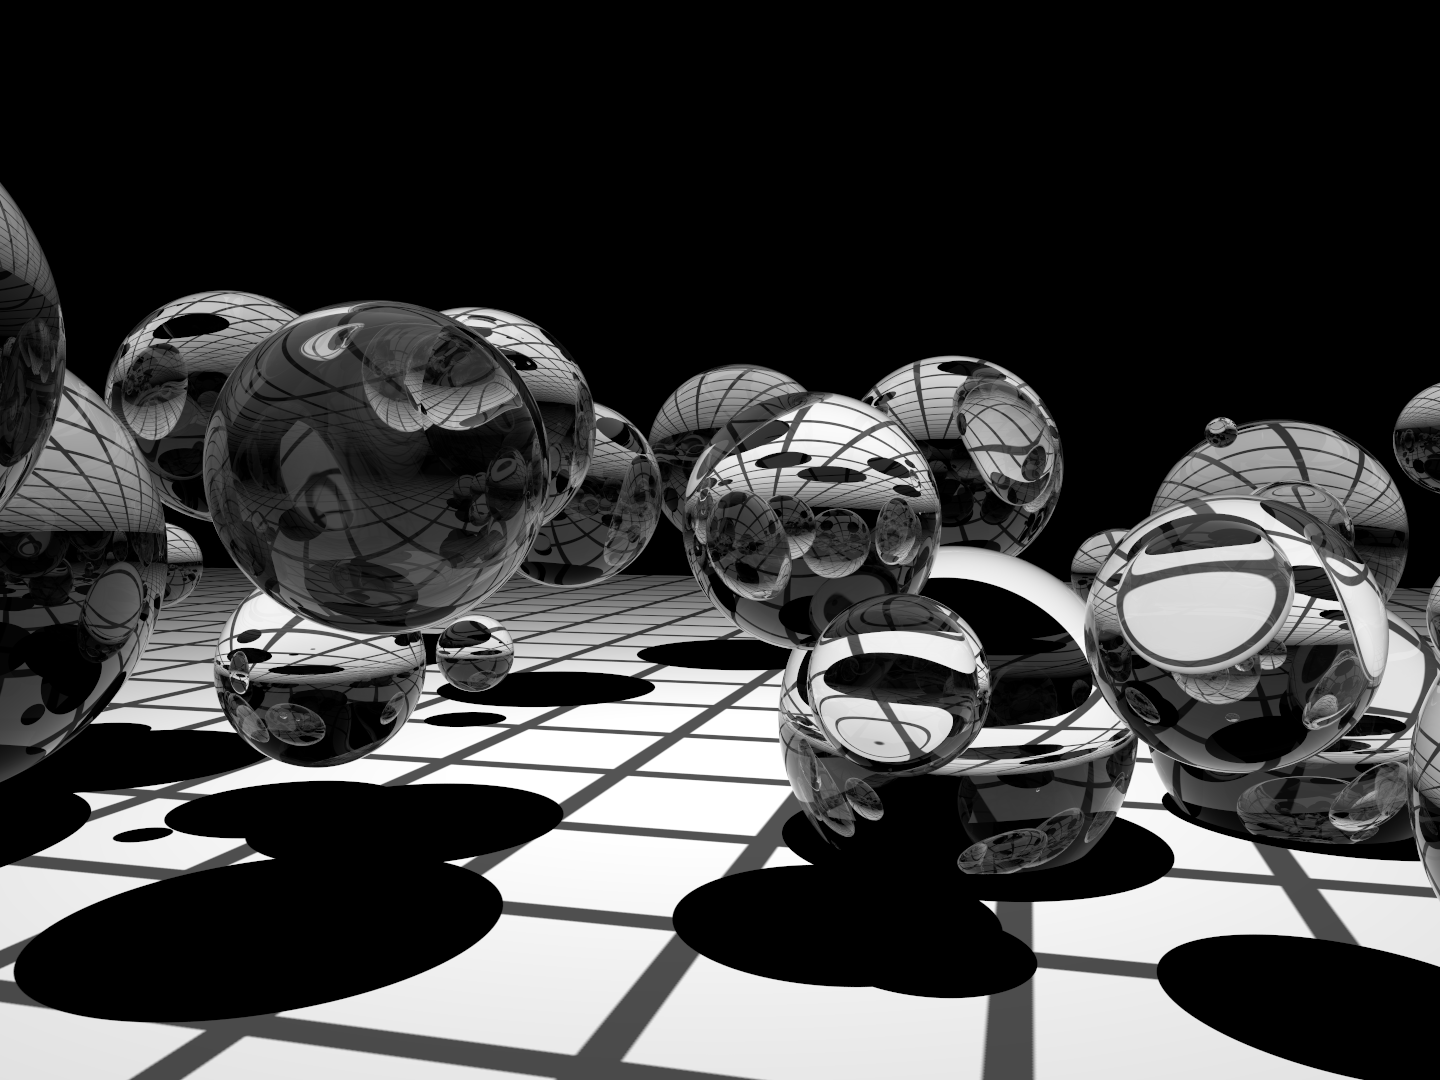
\includegraphics[width=\linewidth]{chap01/spheres-whitted.png}\label{fig:1.7.1}}\\
      \subfloat[随机渐进光子映射。]{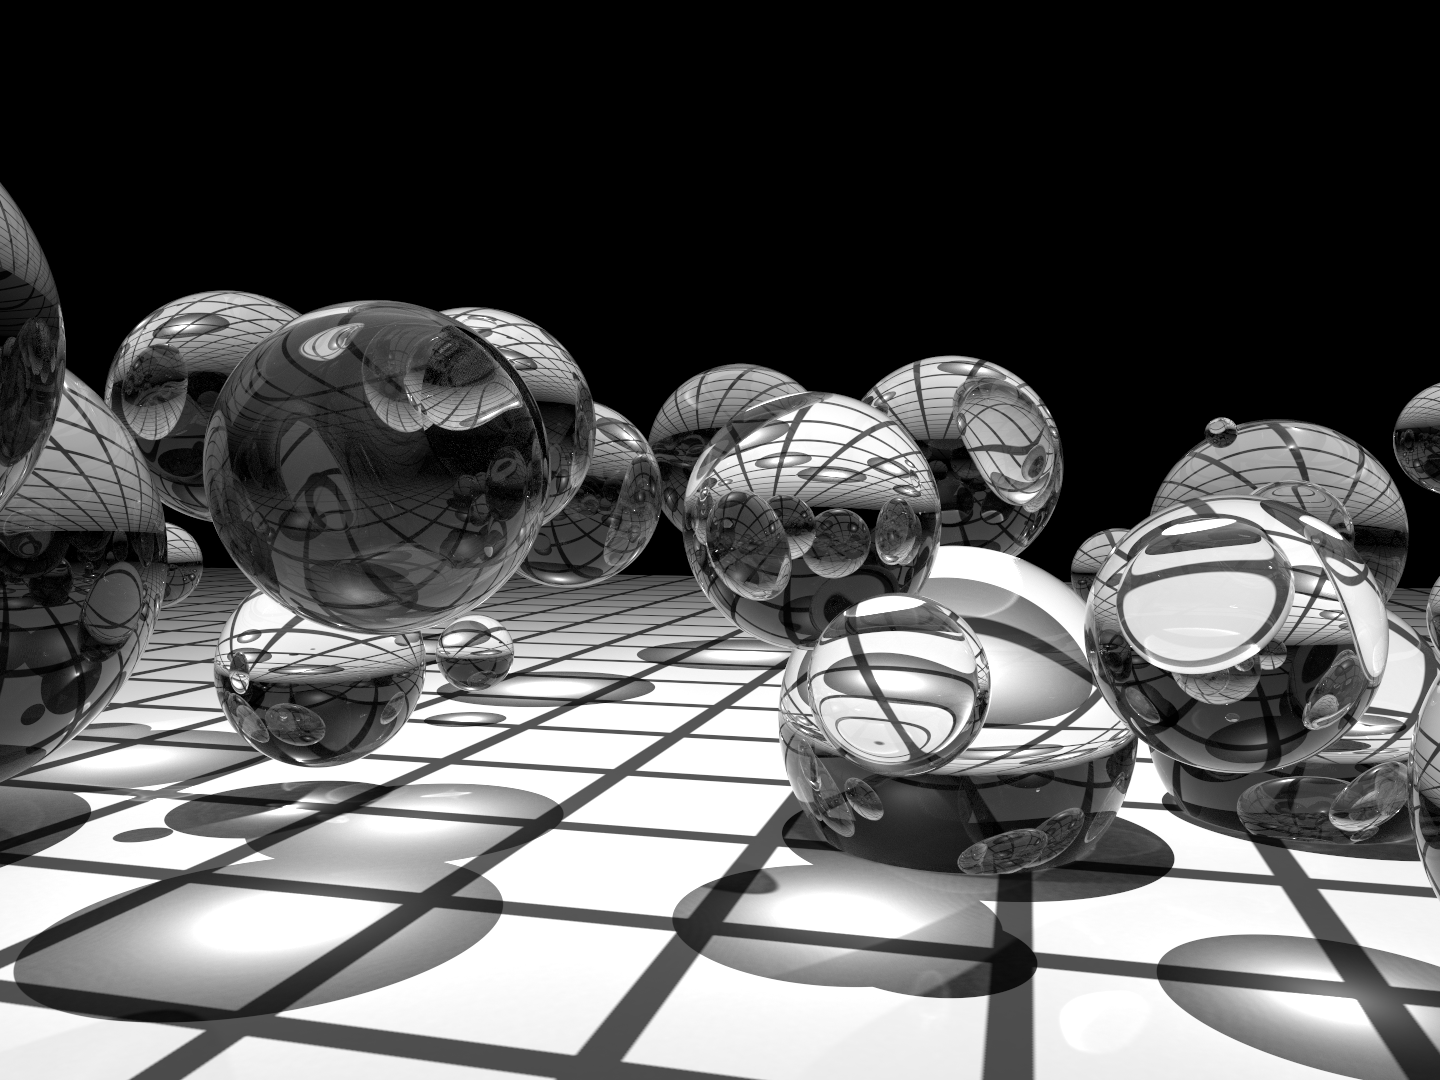
\includegraphics[width=\linewidth]{chap01/spheres-sppm.png}\label{fig:1.7.2}}
      \caption{一个典型的早期光线追踪场景。
            注意镜面和玻璃物体的使用,
            它强调了算法处理这类表面的能力。
            (a)使用Whitted光线追踪渲染,
            (b)使用随机渐进光子映射(SPPM),
            \refsec{随机渐进光子映射}将介绍这一高级光传输算法。
            SPPM能准确模拟光通过球体的聚焦现象。}\label{fig:1.7}
\end{figure}

通常,从物体上一点到达相机的光量
\sidenote{译者注:此处指辐射亮度。}
由物体的发光量(如果它自己就是光源)与反射光量之和决定。
它被形式化为\keyindex{光传输方程}{light transport equation}{light transport光传输}
(也称作\keyindex{渲染方程}{rendering equation}{render渲染}),
表示从点p沿方向$\omega_\mathrm{o}$的
出射辐亮度$L_{\mathrm{o}}(\mathrm{p},\omega_\mathrm{o})$等于
该点沿该方向的发光亮度加上
点p的邻域球面$\mathrm{S}^2$所有方向上
经BSDF$f(\mathrm{p},\omega_\mathrm{o},\omega_\mathrm{i})$和
余弦项调制的入射亮度:
\begin{align}
      L_{\mathrm{o}}(\mathrm{p},\omega_\mathrm{o})=L_{\mathrm{e}}(\mathrm{p},\omega_\mathrm{o})+\int_{\mathrm{S}^2}f(\mathrm{p},\omega_\mathrm{o},\omega_\mathrm{i})L_{\mathrm{i}}(\mathrm{p},\omega_\mathrm{i})|\cos{\theta_{\mathrm{i}}}| \,\mathrm{d}\omega_\mathrm{i}\, .
      \label{eq:1.1}
\end{align}
\refsub{BRDF}和\refsec{光传输方程}将展示其更完整的推导。
除了最简单的场景,
解析地求解该方程是几乎不可能的,
所以必须简化假设或使用数值积分技术。

Whitted算法通过忽略绝大多数方向的入射光来简化积分,
只计算到光源方向以及
完美\keyindex{反射}{reflection}{}与\keyindex{折射}{refraction}{}方向
的$L_{\mathrm{i}}(\mathrm{p},\omega_\mathrm{i})$。
换句话说,它把积分变为少量方向上的求和。

Whitted的方法可以扩展到实现镜面和玻璃外的更多效果。
例如,追踪许多贴近\keyindex{镜面反射}{mirror reflection}{reflection反射}方向
的递归光线并平均它们的作用,
可以近似得到\keyindex{光泽反射}{glossy reflection}{reflection反射}。
事实上只要命中物体我们就\emph{一直}递归地追踪光线。
例如,随机选取反射方向$\omega_\mathrm{i}$并
计算BRDF$f_{\mathrm{r}}(\mathrm{p},\omega_\mathrm{o},\omega_\mathrm{i})$对
这条新建光线赋权。
这个简单有效的办法可以得到非常逼真的图像,
因为它考虑了物体间的光所有的\keyindex{互反射}{interreflection}{reflection反射}。
当然,我们需要知道何时停止递归,
何况完全随机选取方向会让渲染算法收敛到合理结果的速度变慢。
但是这些问题是可以解决的;
第\refchap{蒙特卡洛积分}和第\refchap{光传输III:双向方法}会对这些问题予以介绍。

当用该方法递归追踪光线时,
其实是把光线的一棵\keyindex{树}{tree}{}与图像的每个位置关联(\reffig{1.8}),
来自相机的射线是该树的根。
树中每条光线有关联的\keyindex{权重}{weight}{};
这允许我们对不反射100\%入射光的光滑表面建模。
\begin{figure}
      \centering%LaTeX with PSTricks extensions
%%Creator: Inkscape 1.0.1 (3bc2e813f5, 2020-09-07)
%%Please note this file requires PSTricks extensions
\psset{xunit=.5pt,yunit=.5pt,runit=.5pt}
\begin{pspicture}(299.05999756,247.58999634)
{
\newrgbcolor{curcolor}{0 0 0}
\pscustom[linewidth=1,linecolor=curcolor,linestyle=dashed,dash=2]
{
\newpath
\moveto(241.8999939,170.69999695)
\lineto(38.70000076,201.83999634)
}
}
{
\newrgbcolor{curcolor}{0 0 0}
\pscustom[linewidth=1,linecolor=curcolor,linestyle=dashed,dash=4]
{
\newpath
\moveto(151,105.91999817)
\lineto(27.70999908,199.76999664)
}
}
{
\newrgbcolor{curcolor}{0.98823529 0.93333334 0.12941177}
\pscustom[linestyle=none,fillstyle=solid,fillcolor=curcolor]
{
\newpath
\moveto(36.47,235.24999634)
\lineto(34.1,220.73999634)
\lineto(41.53,233.42999634)
\lineto(36.54,219.59999634)
\lineto(46.17,230.69999634)
\lineto(38.73,218.02999634)
\lineto(50.23,227.16999634)
\lineto(40.58,216.07999634)
\lineto(53.58,222.95999634)
\lineto(42.05,213.82999634)
\lineto(56.09,218.19999634)
\lineto(43.09,211.34999634)
\lineto(57.69,213.05999634)
\lineto(43.64,208.70999634)
\lineto(58.31,207.71999634)
\lineto(43.71,206.02999634)
\lineto(57.94,202.34999634)
\lineto(43.28,203.36999634)
\lineto(56.59,197.13999634)
\lineto(42.37,200.83999634)
\lineto(54.31,192.26999634)
\lineto(41.01,198.51999634)
\lineto(51.17,187.89999634)
\lineto(39.24,196.48999634)
\lineto(47.29,184.17999634)
\lineto(37.13,194.81999634)
\lineto(42.78,181.23999634)
\lineto(34.75,193.55999634)
\lineto(37.81,179.17999634)
\lineto(32.19,192.75999634)
\lineto(32.55,178.05999634)
\lineto(29.51,192.44999634)
\lineto(27.17,177.92999634)
\lineto(26.83,192.62999634)
\lineto(21.86,178.79999634)
\lineto(24.23,193.30999634)
\lineto(16.8,180.61999634)
\lineto(21.79,194.44999634)
\lineto(12.16,183.33999634)
\lineto(19.6,196.01999634)
\lineto(8.1,186.86999634)
\lineto(17.75,197.95999634)
\lineto(4.75,191.07999634)
\lineto(16.27,200.20999634)
\lineto(2.24,195.83999634)
\lineto(15.24,202.69999634)
\lineto(0.64,200.97999634)
\lineto(14.69,205.32999634)
\lineto(0.02,206.31999634)
\lineto(14.62,208.01999634)
\lineto(0.39,211.68999634)
\lineto(15.05,210.67999634)
\lineto(1.73,216.89999634)
\lineto(15.96,213.20999634)
\lineto(4.02,221.76999634)
\lineto(17.32,215.52999634)
\lineto(7.15,226.13999634)
\lineto(19.09,217.55999634)
\lineto(11.04,229.85999634)
\lineto(21.2,219.22999634)
\lineto(15.55,232.79999634)
\lineto(23.57,220.48999634)
\lineto(20.52,234.86999634)
\lineto(26.14,221.27999634)
\lineto(25.78,235.97999634)
\lineto(28.82,221.59999634)
\lineto(31.16,236.10999634)
\lineto(31.5,221.40999634)
\closepath
}
}
{
\newrgbcolor{curcolor}{0 0 0}
\pscustom[linewidth=0.30000001,linecolor=curcolor]
{
\newpath
\moveto(36.47,235.24999634)
\lineto(34.1,220.73999634)
\lineto(41.53,233.42999634)
\lineto(36.54,219.59999634)
\lineto(46.17,230.69999634)
\lineto(38.73,218.02999634)
\lineto(50.23,227.16999634)
\lineto(40.58,216.07999634)
\lineto(53.58,222.95999634)
\lineto(42.05,213.82999634)
\lineto(56.09,218.19999634)
\lineto(43.09,211.34999634)
\lineto(57.69,213.05999634)
\lineto(43.64,208.70999634)
\lineto(58.31,207.71999634)
\lineto(43.71,206.02999634)
\lineto(57.94,202.34999634)
\lineto(43.28,203.36999634)
\lineto(56.59,197.13999634)
\lineto(42.37,200.83999634)
\lineto(54.31,192.26999634)
\lineto(41.01,198.51999634)
\lineto(51.17,187.89999634)
\lineto(39.24,196.48999634)
\lineto(47.29,184.17999634)
\lineto(37.13,194.81999634)
\lineto(42.78,181.23999634)
\lineto(34.75,193.55999634)
\lineto(37.81,179.17999634)
\lineto(32.19,192.75999634)
\lineto(32.55,178.05999634)
\lineto(29.51,192.44999634)
\lineto(27.17,177.92999634)
\lineto(26.83,192.62999634)
\lineto(21.86,178.79999634)
\lineto(24.23,193.30999634)
\lineto(16.8,180.61999634)
\lineto(21.79,194.44999634)
\lineto(12.16,183.33999634)
\lineto(19.6,196.01999634)
\lineto(8.1,186.86999634)
\lineto(17.75,197.95999634)
\lineto(4.75,191.07999634)
\lineto(16.27,200.20999634)
\lineto(2.24,195.83999634)
\lineto(15.24,202.69999634)
\lineto(0.64,200.97999634)
\lineto(14.69,205.32999634)
\lineto(0.02,206.31999634)
\lineto(14.62,208.01999634)
\lineto(0.39,211.68999634)
\lineto(15.05,210.67999634)
\lineto(1.73,216.89999634)
\lineto(15.96,213.20999634)
\lineto(4.02,221.76999634)
\lineto(17.32,215.52999634)
\lineto(7.15,226.13999634)
\lineto(19.09,217.55999634)
\lineto(11.04,229.85999634)
\lineto(21.2,219.22999634)
\lineto(15.55,232.79999634)
\lineto(23.57,220.48999634)
\lineto(20.52,234.86999634)
\lineto(26.14,221.27999634)
\lineto(25.78,235.97999634)
\lineto(28.82,221.59999634)
\lineto(31.16,236.10999634)
\lineto(31.5,221.40999634)
\closepath
}
}
{
\newrgbcolor{curcolor}{0 0 0}
\pscustom[linewidth=1,linecolor=curcolor,linestyle=dashed,dash=2]
{
\newpath
\moveto(226.91000366,112.62998962)
\lineto(242.02000427,171.44999695)
}
}
{
\newrgbcolor{curcolor}{0 0 0}
\pscustom[linewidth=1,linecolor=curcolor]
{
\newpath
\moveto(67.88999939,58.78999329)
\lineto(136.13999939,58.78999329)
}
}
{
\newrgbcolor{curcolor}{0 0 0}
\pscustom[linestyle=none,fillstyle=solid,fillcolor=curcolor]
{
\newpath
\moveto(131.24,53.27999634)
\lineto(135.49,58.77999634)
\lineto(131.24,64.28999634)
\lineto(144.25,58.77999634)
\closepath
}
}
{
\newrgbcolor{curcolor}{0.65098041 0.65098041 0.65098041}
\pscustom[linestyle=none,fillstyle=solid,fillcolor=curcolor]
{
\newpath
\moveto(132.79,54.47999634)
\lineto(142.94,58.77999634)
\lineto(136.13,58.77999634)
\closepath
}
}
{
\newrgbcolor{curcolor}{0.40000001 0.40000001 0.40000001}
\pscustom[linestyle=none,fillstyle=solid,fillcolor=curcolor]
{
\newpath
\moveto(132.79,63.07999634)
\lineto(142.94,58.77999634)
\lineto(136.13,58.77999634)
\closepath
}
}
{
\newrgbcolor{curcolor}{0 0 0}
\pscustom[linewidth=1,linecolor=curcolor,linestyle=dashed,dash=4]
{
\newpath
\moveto(128.44000244,58.84999084)
\lineto(213.77000427,58.84999084)
}
}
{
\newrgbcolor{curcolor}{0.60000002 0.60000002 0.60000002}
\pscustom[linestyle=none,fillstyle=solid,fillcolor=curcolor]
{
\newpath
\moveto(290.14999771,40.33999634)
\curveto(290.14999771,56.59936135)(280.35552771,71.25783813)(265.33410246,77.47967557)
\curveto(250.31270785,83.70150032)(233.02280553,80.26130324)(221.52574779,68.7642455)
\curveto(210.02869005,57.26718776)(206.58849296,39.97728544)(212.81031772,24.95589082)
\curveto(219.03215516,9.93446558)(233.69063194,0.13999557)(249.94999695,0.13999557)
\curveto(266.20936196,0.13999557)(280.86783874,9.93446558)(287.08967618,24.95589082)
\curveto(293.31150093,39.97728544)(289.87130385,57.26718776)(278.37424611,68.7642455)
\curveto(266.87718837,80.26130324)(249.58728605,83.70150032)(234.56589144,77.47967557)
\curveto(219.54446619,71.25783813)(209.74999619,56.59936135)(209.74999619,40.33999634)
\curveto(209.74999619,24.08063133)(219.54446619,9.42215455)(234.56589144,3.2003171)
\curveto(249.58728605,-3.02150765)(266.87718837,0.41868944)(278.37424611,11.91574718)
\curveto(289.87130385,23.41280492)(293.31150093,40.70270724)(287.08967618,55.72410185)
\curveto(280.86783874,70.7455271)(266.20936196,80.5399971)(249.94999695,80.5399971)
\curveto(233.69063194,80.5399971)(219.03215516,70.7455271)(212.81031772,55.72410185)
\curveto(206.58849296,40.70270724)(210.02869005,23.41280492)(221.52574779,11.91574718)
\curveto(233.02280553,0.41868944)(250.31270785,-3.02150765)(265.33410246,3.2003171)
\curveto(280.35552771,9.42215455)(290.14999771,24.08063133)(290.14999771,40.33999634)
\closepath
}
}
{
\newrgbcolor{curcolor}{0 0 0}
\pscustom[linewidth=0.30000001,linecolor=curcolor]
{
\newpath
\moveto(290.14999771,40.33999634)
\curveto(290.14999771,56.59936135)(280.35552771,71.25783813)(265.33410246,77.47967557)
\curveto(250.31270785,83.70150032)(233.02280553,80.26130324)(221.52574779,68.7642455)
\curveto(210.02869005,57.26718776)(206.58849296,39.97728544)(212.81031772,24.95589082)
\curveto(219.03215516,9.93446558)(233.69063194,0.13999557)(249.94999695,0.13999557)
\curveto(266.20936196,0.13999557)(280.86783874,9.93446558)(287.08967618,24.95589082)
\curveto(293.31150093,39.97728544)(289.87130385,57.26718776)(278.37424611,68.7642455)
\curveto(266.87718837,80.26130324)(249.58728605,83.70150032)(234.56589144,77.47967557)
\curveto(219.54446619,71.25783813)(209.74999619,56.59936135)(209.74999619,40.33999634)
\curveto(209.74999619,24.08063133)(219.54446619,9.42215455)(234.56589144,3.2003171)
\curveto(249.58728605,-3.02150765)(266.87718837,0.41868944)(278.37424611,11.91574718)
\curveto(289.87130385,23.41280492)(293.31150093,40.70270724)(287.08967618,55.72410185)
\curveto(280.86783874,70.7455271)(266.20936196,80.5399971)(249.94999695,80.5399971)
\curveto(233.69063194,80.5399971)(219.03215516,70.7455271)(212.81031772,55.72410185)
\curveto(206.58849296,40.70270724)(210.02869005,23.41280492)(221.52574779,11.91574718)
\curveto(233.02280553,0.41868944)(250.31270785,-3.02150765)(265.33410246,3.2003171)
\curveto(280.35552771,9.42215455)(290.14999771,24.08063133)(290.14999771,40.33999634)
\closepath
}
}
{
\newrgbcolor{curcolor}{0 0 0}
\pscustom[linewidth=1,linecolor=curcolor]
{
\newpath
\moveto(213.91999817,59.44999695)
\lineto(142.57000732,112.30999756)
}
}
{
\newrgbcolor{curcolor}{0 0 0}
\pscustom[linestyle=none,fillstyle=solid,fillcolor=curcolor]
{
\newpath
\moveto(149.79,113.80999634)
\lineto(143.09,111.91999634)
\lineto(143.24,104.95999634)
\lineto(136.06,117.12999634)
\closepath
}
}
{
\newrgbcolor{curcolor}{0.65098041 0.65098041 0.65098041}
\pscustom[linestyle=none,fillstyle=solid,fillcolor=curcolor]
{
\newpath
\moveto(147.82,113.76999634)
\lineto(137.11,116.34999634)
\lineto(142.58,112.29999634)
\closepath
}
}
{
\newrgbcolor{curcolor}{0.40000001 0.40000001 0.40000001}
\pscustom[linestyle=none,fillstyle=solid,fillcolor=curcolor]
{
\newpath
\moveto(142.7,106.85999634)
\lineto(137.11,116.34999634)
\lineto(142.58,112.29999634)
\closepath
}
}
{
\newrgbcolor{curcolor}{0 0 0}
\pscustom[linewidth=1,linecolor=curcolor]
{
\newpath
\moveto(213.47000122,59.59999084)
\lineto(230.1499939,125.26999664)
}
}
{
\newrgbcolor{curcolor}{0 0 0}
\pscustom[linestyle=none,fillstyle=solid,fillcolor=curcolor]
{
\newpath
\moveto(234.28,119.14999634)
\lineto(229.99,124.63999634)
\lineto(223.61,121.86999634)
\lineto(232.15,133.11999634)
\closepath
}
}
{
\newrgbcolor{curcolor}{0.65098041 0.65098041 0.65098041}
\pscustom[linestyle=none,fillstyle=solid,fillcolor=curcolor]
{
\newpath
\moveto(233.5,120.95999634)
\lineto(231.82,131.84999634)
\lineto(230.15,125.24999634)
\closepath
}
}
{
\newrgbcolor{curcolor}{0.40000001 0.40000001 0.40000001}
\pscustom[linestyle=none,fillstyle=solid,fillcolor=curcolor]
{
\newpath
\moveto(225.16,123.07999634)
\lineto(231.82,131.84999634)
\lineto(230.15,125.24999634)
\closepath
}
}
{
\newrgbcolor{curcolor}{0.60000002 0.60000002 0.60000002}
\pscustom[linestyle=none,fillstyle=solid,fillcolor=curcolor]
{
\newpath
\moveto(298.90999222,207.23999786)
\curveto(298.90999222,223.49936287)(289.11552221,238.15783966)(274.09409697,244.3796771)
\curveto(259.07270236,250.60150185)(241.78280003,247.16130476)(230.2857423,235.66424702)
\curveto(218.78868456,224.16718929)(215.34848747,206.87728696)(221.57031222,191.85589235)
\curveto(227.79214966,176.8344671)(242.45062645,167.0399971)(258.70999146,167.0399971)
\curveto(274.96935646,167.0399971)(289.62783325,176.8344671)(295.84967069,191.85589235)
\curveto(302.07149544,206.87728696)(298.63129835,224.16718929)(287.13424061,235.66424702)
\curveto(275.63718288,247.16130476)(258.34728055,250.60150185)(243.32588594,244.3796771)
\curveto(228.3044607,238.15783966)(218.50999069,223.49936287)(218.50999069,207.23999786)
\curveto(218.50999069,190.98063285)(228.3044607,176.32215607)(243.32588594,170.10031863)
\curveto(258.34728055,163.87849388)(275.63718288,167.31869097)(287.13424061,178.8157487)
\curveto(298.63129835,190.31280644)(302.07149544,207.60270877)(295.84967069,222.62410338)
\curveto(289.62783325,237.64552862)(274.96935646,247.43999863)(258.70999146,247.43999863)
\curveto(242.45062645,247.43999863)(227.79214966,237.64552862)(221.57031222,222.62410338)
\curveto(215.34848747,207.60270877)(218.78868456,190.31280644)(230.2857423,178.8157487)
\curveto(241.78280003,167.31869097)(259.07270236,163.87849388)(274.09409697,170.10031863)
\curveto(289.11552221,176.32215607)(298.90999222,190.98063285)(298.90999222,207.23999786)
\closepath
}
}
{
\newrgbcolor{curcolor}{0 0 0}
\pscustom[linewidth=0.30000001,linecolor=curcolor]
{
\newpath
\moveto(298.90999222,207.23999786)
\curveto(298.90999222,223.49936287)(289.11552221,238.15783966)(274.09409697,244.3796771)
\curveto(259.07270236,250.60150185)(241.78280003,247.16130476)(230.2857423,235.66424702)
\curveto(218.78868456,224.16718929)(215.34848747,206.87728696)(221.57031222,191.85589235)
\curveto(227.79214966,176.8344671)(242.45062645,167.0399971)(258.70999146,167.0399971)
\curveto(274.96935646,167.0399971)(289.62783325,176.8344671)(295.84967069,191.85589235)
\curveto(302.07149544,206.87728696)(298.63129835,224.16718929)(287.13424061,235.66424702)
\curveto(275.63718288,247.16130476)(258.34728055,250.60150185)(243.32588594,244.3796771)
\curveto(228.3044607,238.15783966)(218.50999069,223.49936287)(218.50999069,207.23999786)
\curveto(218.50999069,190.98063285)(228.3044607,176.32215607)(243.32588594,170.10031863)
\curveto(258.34728055,163.87849388)(275.63718288,167.31869097)(287.13424061,178.8157487)
\curveto(298.63129835,190.31280644)(302.07149544,207.60270877)(295.84967069,222.62410338)
\curveto(289.62783325,237.64552862)(274.96935646,247.43999863)(258.70999146,247.43999863)
\curveto(242.45062645,247.43999863)(227.79214966,237.64552862)(221.57031222,222.62410338)
\curveto(215.34848747,207.60270877)(218.78868456,190.31280644)(230.2857423,178.8157487)
\curveto(241.78280003,167.31869097)(259.07270236,163.87849388)(274.09409697,170.10031863)
\curveto(289.11552221,176.32215607)(298.90999222,190.98063285)(298.90999222,207.23999786)
\closepath
}
}
{
\newrgbcolor{curcolor}{0 0 0}
\pscustom[linewidth=1,linecolor=curcolor]
{
\newpath
\moveto(240.69000244,170.88999939)
\lineto(151.6499939,184.52999496)
}
}
{
\newrgbcolor{curcolor}{0 0 0}
\pscustom[linestyle=none,fillstyle=solid,fillcolor=curcolor]
{
\newpath
\moveto(157.33,189.22999634)
\lineto(152.29,184.42999634)
\lineto(155.67,178.34999634)
\lineto(143.64,185.75999634)
\closepath
}
}
{
\newrgbcolor{curcolor}{0.65098041 0.65098041 0.65098041}
\pscustom[linestyle=none,fillstyle=solid,fillcolor=curcolor]
{
\newpath
\moveto(155.61,188.27999634)
\lineto(144.93,185.55999634)
\lineto(151.66,184.52999634)
\closepath
}
}
{
\newrgbcolor{curcolor}{0.40000001 0.40000001 0.40000001}
\pscustom[linestyle=none,fillstyle=solid,fillcolor=curcolor]
{
\newpath
\moveto(154.31,179.77999634)
\lineto(144.93,185.55999634)
\lineto(151.66,184.52999634)
\closepath
}
}
\end{pspicture}

      \caption{递归光线追踪与一整棵关于图像每处位置光线的树关联。}\label{fig:1.8}
\end{figure}

\subsection{光线传播}\label{sub:光线传播}

目前的讨论都假设光线是在\keyindex{真空}{vacuum}{}中传播的。
例如在描述点光源的光分布时,
我们假设光的功率朝着
以光源为球心的球面均匀发散且不随路线衰减
\sidenote{译者注:意思是没有传播介质吸收光的能量,
      和前文反比于半径平方不是一回事。}。
\keyindex{介质}{participating media}{}的出现,
例如烟、雾、尘会破坏该假设。
模拟这些效果很重要:
即使我们不渲染充满烟气的房间,
几乎所有室外场景也都会受到介质的实质影响。
例如,地球大气使得远处物体显得不够饱和(\reffig{1.9})。
\begin{figure}
      \centering
      \subfloat[无大气散射]{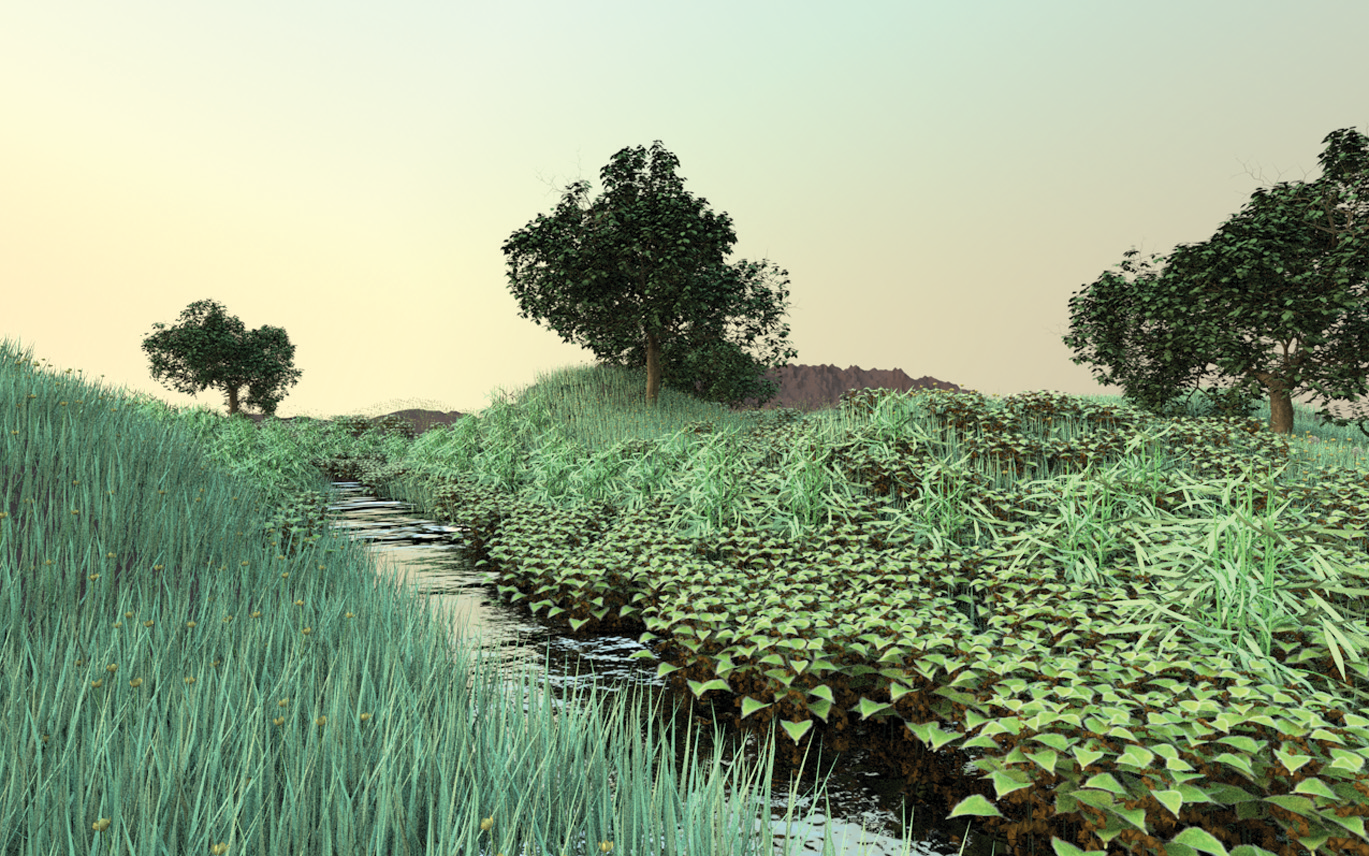
\includegraphics[width=\linewidth]{chap01/ecosys-nofog.png}\label{fig:1.9.1}}\\
      \subfloat[有大气散射]{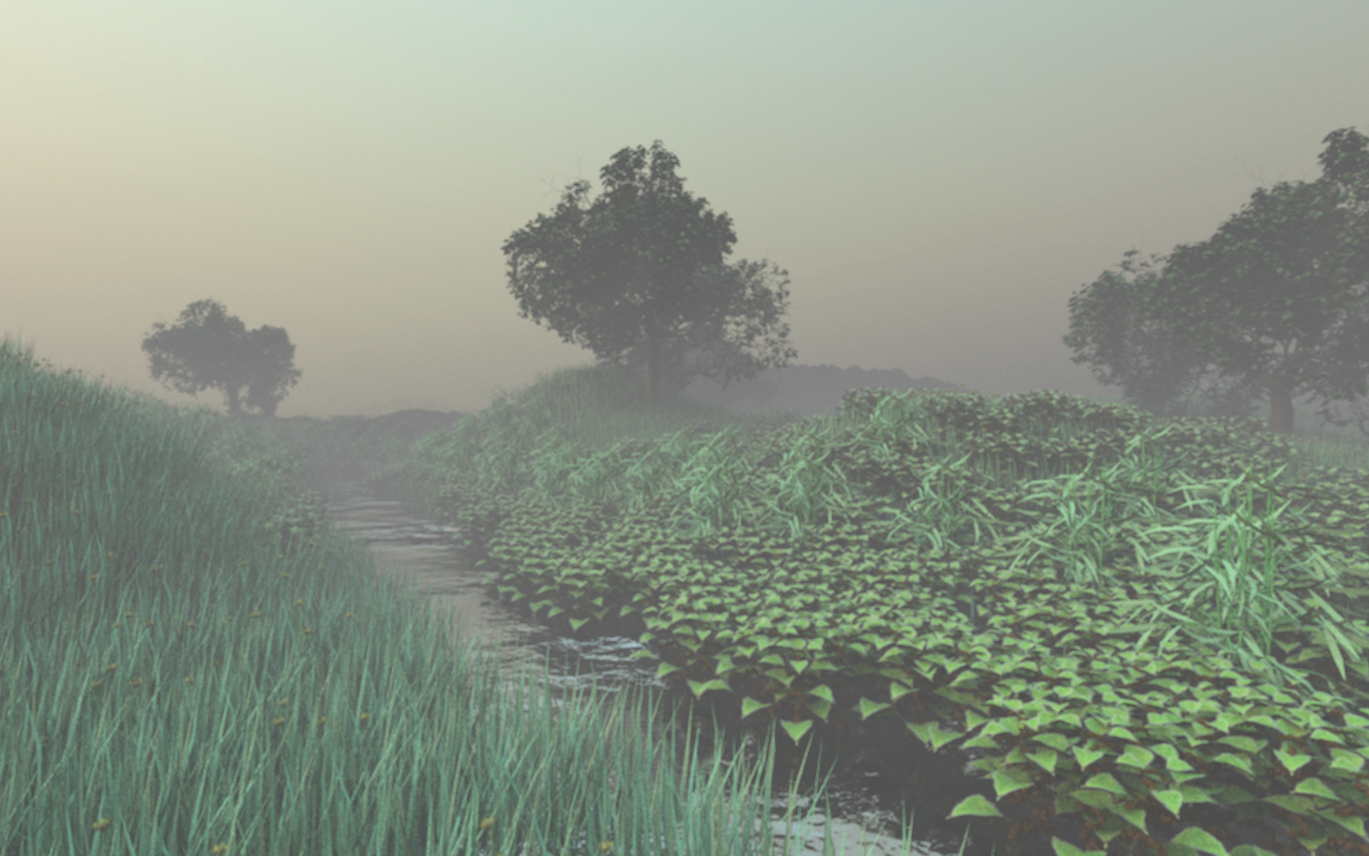
\includegraphics[width=\linewidth]{chap01/ecosys-fog.png}\label{fig:1.9.2}}
      \caption{地球大气随距离降低饱和度。
            (a)渲染场景没有模拟该现象,但(b)包含了大气模型。
            大气衰减程度是观察真实场景时重要的深度线索,
            为二次渲染增加了尺度感。}
      \label{fig:1.9}
\end{figure}

介质影响光沿路线传播的方式有两种。
第一种是介质可以通过吸收或沿不同方向散射
来\keyindex{熄灭}{extinguish}{}(或\keyindex{衰减}{attenuate}{})光。
可以通过计算射线端点与交点之间的\keyindex{透射率}{transmittance}{}$T$来
实现这一效果。
透射率表示交点处散射的光有多少成功到达射线端点。

介质也可以沿路线增强光。
在介质发光(例如火焰)或从其他方向把光散射回该射线时可发生该现象(\reffig{1.10})。
可以通过数值计算\keyindex{体积光传输方程}{volume light transport equation}{light transport光传输}来寻求该量,
该方法还能计算光传输方程求得从表面反射回的光量。
介质的描述和体积渲染会留到第\refchap{体积散射}和\refchap{光传输II:体积渲染}。
现在我们就能计算介质效应并将其合并到光线所含的光量中了。
\begin{figure}
      \centering
      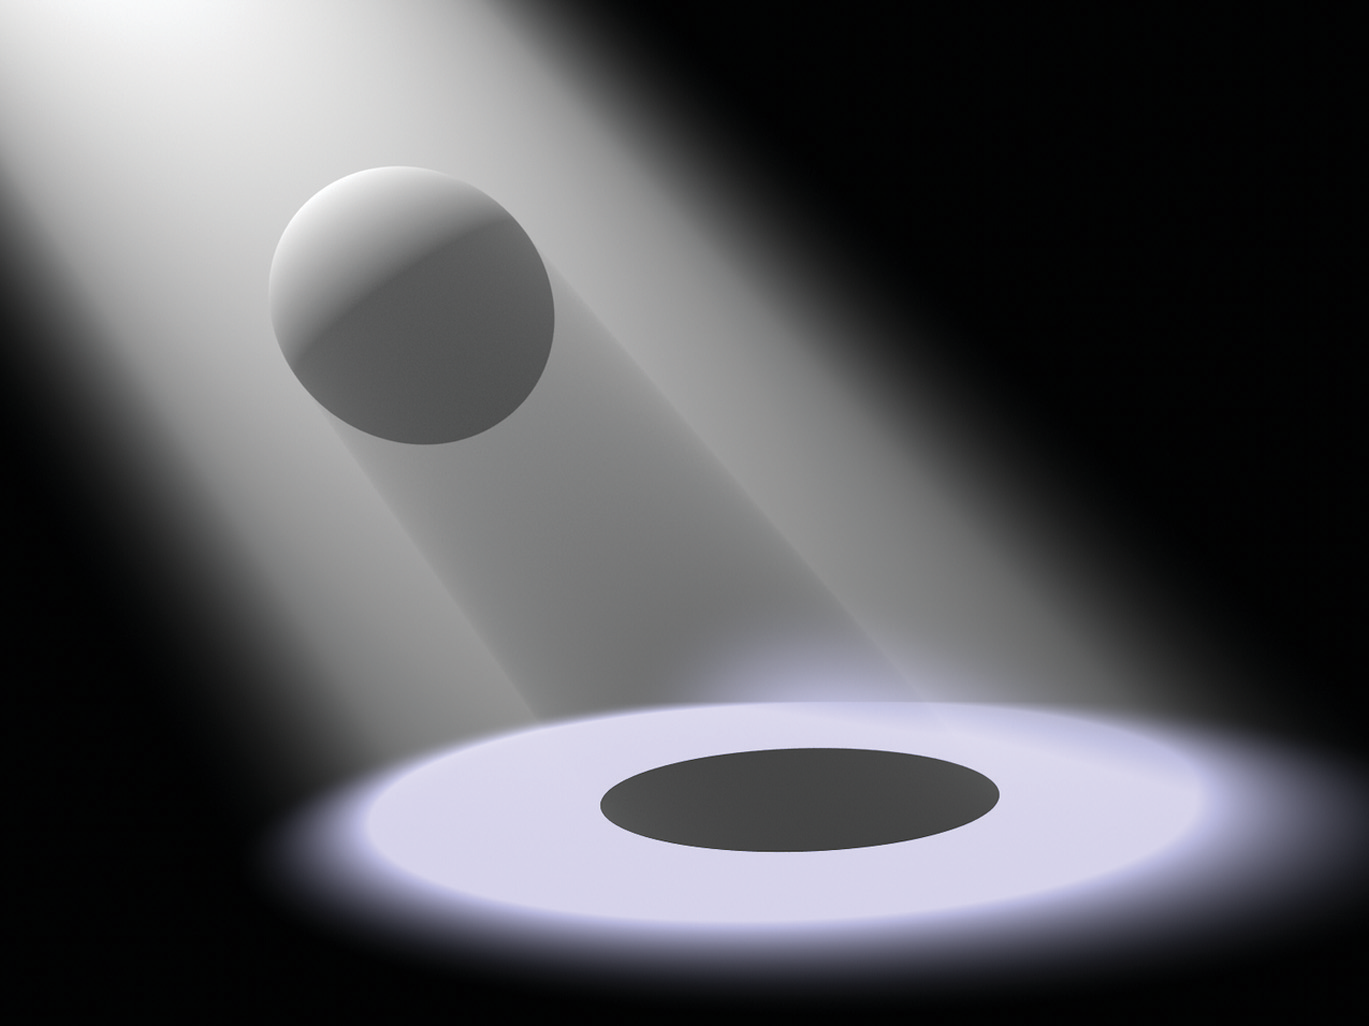
\includegraphics[width=\linewidth]{chap01/spotfog.png}
      \caption{聚光灯通过雾气照在球上。
            注意因为介质增加了散射,聚光灯的光分布形状和球的阴影清晰可见。}
      \label{fig:1.10}
\end{figure}